% !TeX root = OVATiK.tex
\documentclass[11pt,a4paper]{article}
%\documentclass[a4paper,12pt, draft]{article}

%%% Работа с русским языком
\usepackage{cmap}					% поиск в PDF
\usepackage{mathtext} 				% русские буквы в формулах
\usepackage[T2A]{fontenc}			% кодировка
\usepackage[utf8]{inputenc}			% кодировка исходного текста
\usepackage[english,russian]{babel}	% локализация и переносы
\usepackage{indentfirst}            % красная строка в первом абзаце
\frenchspacing                      % равные пробелы между словами и предложениями
% 
%%% Дополнительная работа с математикой
\usepackage{amsmath,amsfonts,amssymb,amsthm,mathtools} % пакеты AMS
\usepackage{icomma}                                    % "Умная" запятая
% \usepackage{unicode-math} % русский в математике
\usepackage{gensymb} % градус



%%% Свои символы и команды
\usepackage{centernot} % центрированное зачеркивание символа
\usepackage{stmaryrd}  % некоторые спецсимволы
\usepackage{dsfont}
\usepackage{amsthm}

\renewcommand{\epsilon}{\ensuremath{\varepsilon}}
\renewcommand{\phi}{\ensuremath{\varphi}}
\renewcommand{\kappa}{\ensuremath{\varkappa}}
\renewcommand{\le}{\ensuremath{\leqslant}}
\renewcommand{\leq}{\ensuremath{\leqslant}}
\renewcommand{\ge}{\ensuremath{\geqslant}}
\renewcommand{\geq}{\ensuremath{\geqslant}}
\renewcommand{\emptyset}{\ensuremath{\varnothing}}
% \renewcommand{\c}{\cdot}

\DeclareMathOperator{\sgn}{sgn}
\DeclareMathOperator{\ord}{ord}
\DeclareMathOperator{\lcm}{\text{НОК}}
\DeclareMathOperator{\gcdru}{\text{НОД}}
\DeclareMathOperator{\ke}{Ker}
\DeclareMathOperator{\im}{Im}
\DeclareMathOperator{\re}{Re}
\DeclareMathOperator{\orb}{Orb}
\DeclareMathOperator{\stab}{Stab}
\DeclareMathOperator{\charf}{char}
\DeclareMathOperator{\eva}{Eva}


\newcommand{\NN}{\mathbb{N}}
\newcommand{\ZZ}{\mathbb{Z}}
\newcommand{\QQ}{\mathbb{Q}}
\newcommand{\RR}{\mathbb{R}}
\newcommand{\Cm}{\mathbb{C}}
\newcommand{\FF}{\mathbb{F}}
\newcommand{\id}{\mathrm{id}}


\newcommand{\comp}{\circ}
\newcommand{\raone}{\mapsto}
\newcommand{\Ra}{\Rightarrow}
\newcommand{\ra}{\rightarrow}
\newcommand{\hra}{\hookrightarrow}
\newcommand{\La}{\Leftarrow}
\newcommand{\la}{\leftarrow}
\newcommand{\Lra}{\Leftrightarrow}
\newcommand{\lra}{\leftrightarrow}
\renewcommand{\subset}{\subseteq}
\newcommand{\sub}{\subset}
\newcommand{\sconstr}{\;\vert\;}
\newcommand{\thus}{\implies}
\newcommand{\cd}{\cdot}

% \newcommand{\myeq{\stackrel{\mathclap{\normalfont\mbox{def}}}{=}}}
\newcommand{\defeq}{\vcentcolon= }
\newcommand{\defev}{\stackrel{\Delta}{\Longleftrightarrow}}
% \newcommand{\deriv}[3][1]{%
% 	\ifthenelse{#1>1}{%
% 		\frac{\delta^{#1} {#2}}{\delta {#3}^{#1}}
% 	}{%
% 		\frac{\delta {#2}}{\delta {#3}}
% 	}%
% }
\newcommand{\deriv}[3]{\frac{\delta^{#1} {#2}}{\delta {#3}^{#1}}}

\renewcommand{\labelitemi}{$\triangleright$}

% \equalto --- делает вертикальное равно
\newcommand{\verteq}{\rotatebox{90}{$\,=$}}
\newcommand{\equalto}[2]{\underset{\scriptstyle\overset{\mkern4mu\verteq}{#2}}{#1}}


% \let\bs\backslash
% \let\lra\Leftrightarrow
% \let\ra\Rightarrow
% \let\la\Leftarrow
% \let\emb\hookrightarrow

%%% Перенос знаков в формулах (по Львовскому)
\newcommand{\hm}[1]{#1\nobreak\discretionary{}{\hbox{$\mathsurround=0pt #1$}}{}}

%%% Работа с картинками
\usepackage{graphicx}    % Для вставки рисунков
\setlength\fboxsep{3pt}  % Отступ рамки \fbox{} от рисунка
\setlength\fboxrule{1pt} % Толщина линий рамки \fbox{}
\usepackage{wrapfig}     % Обтекание рисунков текстом

%%% Работа с таблицами
\usepackage{array,tabularx,tabulary,booktabs} % Дополнительная работа с таблицами
\usepackage{longtable}                        % Длинные таблицы
\usepackage{multirow}                         % Слияние строк в таблице

%%% Теоремы
\theoremstyle{plain}
\newtheorem*{theorem}{Теорема}
\newtheorem*{lemma}{Лемма}
\newtheorem*{proposition}{Утверждение}
\newtheorem*{exercise}{Упражнение}
\newtheorem*{problem}{Задача}

\theoremstyle{definition}
\newtheorem*{definition}{Определение}
\newtheorem*{corollary}{Следствие}
\newtheorem*{note}{Замечание}
\newtheorem*{reminder}{Напоминание}
\newtheorem*{example}{Пример}

\theoremstyle{remark}
\newtheorem*{solution}{Решение}

%%% Оформление страницы
\usepackage{extsizes}     % Возможность сделать 14-й шрифт
\usepackage{geometry}     % Простой способ задавать поля
\usepackage{setspace}     % Интерлиньяж
\usepackage{enumitem}     % Настройка окружений itemize и enumerate
\setlist{leftmargin=20pt} % Отступы в itemize и enumerate

\geometry{top=25mm}    % Поля сверху страницы
\geometry{bottom=30mm} % Поля снизу страницы
\geometry{left=20mm}   % Поля слева страницы
\geometry{right=20mm}  % Поля справа страницы

\setlength\parindent{15pt}        % Устанавливает длину красной строки 15pt
\linespread{1}                  % Коэффициент межстрочного интервала
%\setlength{\parskip}{0.5em}      % Вертикальный интервал между абзацами
\setcounter{secnumdepth}{0}      % Отключение нумерации разделов
%\setcounter{section}{-1}         % Нумерация секций с нуля
\usepackage{multicol}			  % Для текста в нескольких колонках
\usepackage{soulutf8}             % Модификаторы начертания
\mathtoolsset{showonlyrefs=true} % показывать номера формул только у тех, у которых есть ссылки по eqref
%%% Содержаниие
\usepackage{tocloft}
\tocloftpagestyle{main}
%\setlength{\cftsecnumwidth}{2.3em}
%\renewcommand{\cftsecdotsep}{1}
%\renewcommand{\cftsecpresnum}{\hfill}
%\renewcommand{\cftsecaftersnum}{\quad}

%%% Шаблонная информация для титульного листа
\newcommand{\CourseName}{Основы Высшей Алгебры и Теории Кодирования}
\newcommand{\FullCourseNameFirstPart}{\so{ОСНОВЫ ВЫСШЕЙ АЛГЕБРЫ И ТЕОРИИ КОДИРОВАНИЯ}}
\newcommand{\SemesterNumber}{II}
\newcommand{\LecturerInitials}{Вялый Михаил Николаевич}
\newcommand{\CourseDate}{Весна 2023}
\newcommand{\AuthorInitials}{Юдин Иван}
\newcommand{\VKLink}{https://vk.com/prk_gufik}
\newcommand{\GithubLink}{https://github.com/daniild71r/lectures_tex_club}

%%% Колонтитулы
\usepackage{titleps}
\newpagestyle{main}{
	\setheadrule{0.4pt}
	\sethead{\CourseName}{}{\hyperlink{intro}{\;Назад к содержанию}}
	\setfootrule{0.4pt}                       
	\setfoot{ФПМИ МФТИ, \CourseDate}{}{\thepage} 
}
\pagestyle{main}  

%%% Нумерация уравнений
\makeatletter
\def\eqref{\@ifstar\@eqref\@@eqref}
\def\@eqref#1{\textup{\tagform@{\ref*{#1}}}}
\def\@@eqref#1{\textup{\tagform@{\ref{#1}}}}
\makeatother                      % \eqref* без гиперссылки
\numberwithin{equation}{section}  % Нумерация вида (номер_секции).(номер_уравнения)
\mathtoolsset{showonlyrefs= true} % Номера только у формул с \eqref{} в тексте.

%%% Гиперссылки
\usepackage{hyperref}
\usepackage[usenames,dvipsnames,svgnames,table,rgb]{xcolor}
\hypersetup{
	unicode=true,            % русские буквы в раздела PDF
	colorlinks=true,       	 % Цветные ссылки вместо ссылок в рамках
	linkcolor=black!15!blue, % Внутренние ссылки
	citecolor=green,         % Ссылки на библиографию
	filecolor=magenta,       % Ссылки на файлы
	urlcolor=NavyBlue,       % Ссылки на URL
}

%%% Графика
\usepackage{tikz}        % Графический пакет tikz
\usepackage{tikz-cd}     % Коммутативные диаграммы
\usepackage{tkz-euclide} % Геометрия
\usepackage{stackengine} % Многострочные тексты в картинках
\usetikzlibrary{angles, babel, quotes}

\begin{document}
    \begin{titlepage}
	\clearpage\thispagestyle{empty}
	\centering
	
	\textbf{Московский физико-технический институт \\ Физтех-школа прикладной математики и информатики}
	\vspace{33ex}
	
	{\textbf{\FullCourseNameFirstPart}}
	
	\SemesterNumber\ СЕМЕСТР  
	\vspace{1ex}
	
	Лектор: \textit{\LecturerInitials}
	
	
\includegraphics[width=0.4\textwidth]{images/logo_ltc.png}

	\begin{flushright}
		\noindent
		Автор:  \href{\VKLink}{\textit{\AuthorInitials}}, \href{\VKLinksecond}{\textit{\AuthorInitialssecond}}

		\href{\GithubLink}{\textit{Проект на Github}}
	\end{flushright}
	
	\vfill
	\CourseDate
	\pagebreak
\end{titlepage}

    \newpage
    \hypertarget{intro}{}
    \tableofcontents
    \linespread{1}
    \selectfont

    \newpage
    \section{1. Кольцо многочленов над полем. Наибольший общий делитель. Алгоритм Евклида. Линейное выражение НОД.}

\begin{reminder}
    \textit{Кольцом} называется множество $R$ с определенными на нем бинарными операциями \textit{сложения} $+ : R \times R \to R$ и \textit{умножения} $\cdot: R \times R \rightarrow R$, удовлетворяющими следующим условиям:
    \begin{itemize}
        \item $(R, +)$ "--- абелева группа, нейтральный элемент в которой обозначается через $0$
        \item $\forall a, b, c \in R: (ab)c = a(bc)$ (ассоциативность умножения)
        \item $\forall a, b, c \in R: a(b + c) = ab + ac$ и $(a + b)c = ac + bc$ (дистрибутивность умножения относительно сложения)
    \end{itemize}
\end{reminder}

\begin{reminder}
    \textit{Полем} называется такое коммутативное кольцо $(F, +, \cdot)$, для которого выполнено равенство $F^* = F\backslash\{0\}$.
\end{reminder}

\begin{definition}
    Последовательность $(a_0, a_1, a_2,\ldots), a_i \in R$ называют \textit{финитной} если 
    $\exists N : \forall n>N \hookrightarrow a_n = 0$, т.е. если начиная с некоторого номера $N$ все значения $a_n$ равны нулю.
\end{definition}

\begin{definition}
    Пусть R -- коммутативное кольцо с единицей. \textit{Многочлен} над R -- финитная последовательность элементов A = $(a_0, a_1, a_2,\ldots), a_i \in R$. Дополнительно будем использовать обозначение $(A)_i = a_i$.
\end{definition}

\begin{definition}
    $R[x]$ -- множество многочленов над кольцом R.
\end{definition}

\begin{definition}
    Пусть $A, B \in R[x]$, тогда верны следующие свойства:
    \begin{enumerate}
        \item $(A + B)_n = (A)_n + (B)_n$,
        \item $(A \cdot B)_n = \displaystyle\sum_{i = 0}^{n}(A)_i \cdot (B)_{n-i}$,
        \item $\lambda \in R \; (\lambda A)_n = \lambda \cdot (A)_n$.
    \end{enumerate}
\end{definition}

\begin{proposition}
    Множество всех многочленов R[x] является коммутативным кольцом с 1. $1 = (1, 0, 0,\ldots)$ -- нейтральный по умножению многочлен.
\end{proposition}

\begin{definition}
    Введем обозначения $x = (0, 1, 0, 0, \ldots)$, $x^2 = (0, 0, 1, 0, \ldots)$ и т.д. Тогда многочлен $A = (a_0, a_1, a_2, \ldots)$ можно записать как $A = a_0 \cdot 1 + a_1 \cdot x + a_2 \cdot x^2 + \ldots$.
\end{definition}

\begin{definition}
    Пусть $P = (a_0, a_1, a_2, \ldots)$ -- многочлен. Последний отличный от нуля коэффициент называется \textit{старшим коэффициентом} многочлена. Номер старшего коэффициента называется степенью многочлена и обозначается как $\deg P$.
\end{definition}

\begin{note}
    Будем считать, что степень нулевого многочлена и только нулевого многочлена не определена.
\end{note}

\begin{reminder}
    Делителями нуля называются такие числа $a$ и $b$, что $a \neq 0$ и $b \neq 0$ но $a \cdot b = 0$.
\end{reminder}

\begin{definition}
    Коммутативное кольцо с единицей называется областью целостности или целостным кольцом если оно 
    не имеет делителей нуля.
\end{definition}

\begin{proposition} 
    В области целостности выполняется правило сокращения:
    $ab = ac, a \neq 0 \Rightarrow b = c$.
\end{proposition}

\begin{proof}
    $a(b-c) = 0$, $a \neq 0 \Rightarrow b-c = 0$.
\end{proof}

\begin{proposition}
    Пусть R -- коммутативное кольцо с единицей, $A, B \in R[x]$, тогда:
    \begin{enumerate}
        \item $\deg(A+B) \leq max(\deg(A), \deg(B))$,
        \item $\deg(A \cdot B) \leq \deg(A) + \deg(B)$,
        \item Если вдобавок R -- область целостности, то $\deg(AB) = \deg(A) + \deg(B)$.
    \end{enumerate}
\end{proposition}

\begin{proof}
    \begin{enumerate}
        \item Обозначим $\deg A = a$, $\deg B = b$. Пусть $n > max(a, b)$, тогда
        $(A+B)_n = (A)_n + (B)_n = 0 + 0 = 0$, а значит $\forall n > max(a, b) \Rightarrow (A+B)_n = 0$. 
        Тогда номер последнего ненулевого элемента не превосходит $max(a, b)$, а значит 
        $deg(A+B) \leqslant max(a, b)$

        \item Пусть $n > a + b$, покажем что $(AB)_n = 0$:
        
        $$(AB)_n = \sum_{i = 0}^{a}(A_i)(B_{n-i}) + \sum_{i = a+1}^{n}(A_i)(B_{n-i}) = 0 + 0 = 0$$

        В первой сумме $B_{n-i} = 0$ во всех слагаемых так как $n > a + b$, а значит $n - i > b$ для
        всех $i$ от $0$ до $a$. Во второй сумма во всех слагаемых $A_i = 0$ так как $i > a$ на всем
        диапазоне суммирования. Таким образом обе суммы равны нулю, а значит $(AB)_n = 0$.

        \item Положим $n = a + b$, тогда:
        
        $$(AB)_{n} = \sum_{i=0}^{a-1} (A)_i(B)_{n-i} + (A)_a(B)_b + \sum_{i=a+1}^{a+b} (A)_i(B)_{n-i}$$

        Аналогично предыдущему пункту первое и третье слагаемое будут нулевыми. 
        При этом $(A)_i \neq 0$ и $(B)_{n-i} = (B)_b \neq 0$,  и в силу целостности 
        $((A)_i(B)_{n-i} \neq 0)$, то есть $(AB)_{n} \neq 0$. Для больших
        чем $n$ номеров сумма будет нулевой из предыдущего пункта, а значит $\deg AB = a$.
    \end{enumerate}
\end{proof}

\begin{theorem}[о существовании деления с остатком]
    Пусть $A, B \in F[x]$, F -- поле, $B \neq 0$. Тогда:
    \begin{enumerate}
        \item Cуществуют $Q, R \in F[x]$ т.ч. $A = QB + R$, где $R = 0$ или $\deg R < \deg B$.
        \item Многочлены R и Q определены однозначно.
    \end{enumerate}
\end{theorem}

\begin{proof}~
    \begin{enumerate}
        \item Индукция по $\deg A$:
    
        Пусть $A = 0$ или $\deg A < \deg B$, тогда очевидно $A = 0 \cdot B +A$.

        Пусть теперь $\deg A \geq \deg B$, и они равны a и b соответственно. Тогда старшие 
        члены равны $HT(A) = \alpha x^a$ и $HT(B) = \beta x^b$. Подберем моном M такой что 
        $HT(A) = M \cdot HT(B)$, например $M = \frac{\alpha}{\beta} \cdot x^{a - b}$.

        Введем обозначение $A' = A - MB$, $\deg A' < \deg A$ по построению $M$. По предположению 
        $A' = Q'B + R'$, где $R' = 0$ или $\deg R' < \deg B$. Тогда 
        $A = A' + MB = Q'B + MB + R' = (Q' + M)B + R'$ -- искомое разложение.

        \item Предположим существуют два разложения $A = Q_1 B + R_1 = Q_2 B + R_2$, многочлены 
        удовлетворяют условиям. 

        $(Q_1 - Q_2)B = R_2 - R_1$. Предположим $Q_1 \neq Q_2$, тогда $\deg((Q_1 - Q_2)B) \geq \deg(B)$.
        При этом $\deg (R_2 - R_1) < \deg B$, а значит мы пришли к противоречию и $Q_1 = Q_2$ 
        и $R_1 = R_2$. 
    \end{enumerate}
\end{proof}

\begin{definition}
    $A$ делится на $B$, если существует такой многочлен $Q$ что $A = QB$. Пишут $A \vdots B$ или 
    $B \vert A$.
\end{definition}

\begin{definition}
    Пусть $f(x)$ и $g(x) \in F[x]$ -- не нулевые одновременно многочлены. Многочлен $d(x) \in F[x]$ 
    называется наибольшим общим делителем (НОД, gcd) если:
    \begin{enumerate}
        \item $d \vert f$, $d \vert g$.
        \item если $d'$ -- общий делитель $f$ и $g$, то $d' \vert d$.
    \end{enumerate}

    Иначе говоря, $\gd(f, g)$ -- такой общий делитель, который делится на любой общий делитель.
\end{definition}

\begin{theorem}[алгоритм Евклида, линейное выражение НОД]
    Пусть $f, g \in F[x]$ и $f, g$ ненулевые одновременно. Тогда существует 
    $d(x) = \gd(f, g) \in F[x]$ и, более того, существуют 
    $u(x), v(x) \in F(x)$, такие что $u(x)f(x) + v(x)g(x) = d(x)$.
\end{theorem}

\begin{proof}
    Пусть без ограничения общности $f(x) = 0$, $g(x) \neq 0$. Тогда $d(x) = g(x)$, $d = 0\cdot f + 1\cdot g$.

    Пусть теперь оба многочлена ненулевые. Тогда можно выполнить цепочку делений многочленов, где 
    на каждом новом шаге делимым и делителем будут становиться делитель и частное предыдущего деления
    соответственно. Таким образом для каждой пары НОД будет сохраняться, так как если делитель кратен 
    некоторому многочлену, то делимое и частное будут кратны ему одновременно. Первые несколько шагов:
    \begin{align*}
        f(x)   & = q_1(x)g(x) + r_1(x), \\
        g(x)   & = q_2(x)r_1(x) + r_2(x), \\
        r_1(x) & = q_3(x)r_2(x) + r_3(x). \\
    \end{align*}
    Продолжая действовать так дойдем до последних двух шагов, после которых остаток будет равен нулю.
    При делении степень остатка меньше степени делителя, а значит, в силу конечности номеров старших 
    членов начальных многочленов, в некоторый момент процесс действительно остановится:
    \begin{align*}
        r_{n-2}(x) & = q_n(x)r_{n-1}(x) + r_n(x), \\
        r_{n-1}(x) & = q_{n+1}(x)r_{n}(x).
    \end{align*}
    Получается, что $\gd(f, g)$ = $r_n$ -- последний ненулевой остаток. Проверим:
    \begin{enumerate}
        \item $r_n \vert r_{n-1}$, $r_n \vert r_{n-2}, \ldots$. 
        Продолжая подниматься наверх, получаем $r_n \vert f$, $r_n \vert g$
        \item Теперь будем спускаться вниз, пусть $d' \vert f$, $d' \vert g$. 
        Таким образом мы дойдем до $d' \vert d$.
    \end{enumerate}
    Покажем, что все остатки $r_1, r_2, \ldots, r_n$ являются линейными комбинациями $f$ и $g$:
    $$r_1 = f - q_1g$$
    $$r_2 = g - q_2r_1 = -q_2f + (1 + q_1q_2)g$$
    Спускаясь вниз и подставляя выражения предыдущих остатков в последующие, получим все разложения.
    Положим $r_{n-2} = u''f + v''g$ и $r_{n-1} = u'f + v'g$. Тогда:
    $$d = r_n = r_{n-2} - q_n r_{n-1} = f(u'' - u'q_n) + g(v'' - v'g_n).$$
    Таким образом, все остатки можно выразить через $f$ и $g$.
\end{proof}


    \newpage
    \section{Вопросы из билетов}

\subsection{Эквивалентность фундированности, отсутствия бесконечно убывающей последовательности элементов и принципа трансфинитной индукции.}
\noindent Мы будем работать с частично упорядоченным множеством $(A, \leqslant)$ и для краткости будем его просто называть множеством $A$.
\newline \par \textbf{Теорема:} Три определения фундированного множества эквивалентны друг другу:
\begin{enumerate}
    \item Множество $A$ называется фундированным, если в любом непустом подмножестве $A$ есть минимальный элемент.

    \item Множество $A$ называется фундированным, если для него выполняется принцип невозможности бесконечного спуска: не существует бесконечной строго убывающей последовательности $x_1>x_2>x_3>\ldots$
    
    \item Множество $A$ называется фундированным, если для него выполняется принцип трансфинитной индукции: для любого свойства $\phi(x)$ верно условие:
    $$\forall x \; (\forall y<x \;\; \phi(y)\to \phi(x) ) \;\Rightarrow\; \forall x \phi(x).$$
\end{enumerate}

$\blacktriangle$ (1 $\Rightarrow$ 2) Предположим, что 2 определение неверно, и в множестве есть бесконечная убывающая цепь $x_1 > x_2>\ldots$. Но тогда в множестве $B = \{x_1, x_2, \ldots\}$ нет минимального элемента, что противоречит определению 1.

\par 
(2 $\Rightarrow$ 1) Теперь предположим, что определение 1 не выполнено. Это значит, что в $A$ есть непустое подмножество $B$, в котором нет минимального элемента. Поскольку $B\neq \emptyset$, то $\exists x_1\in B$. Мы предположили, что в $B$ нет минимальных элементов. В частности, $x_1\neq min$, то $\exists x_2 < x_1$. Поскольку $x_2\neq min$, то $\exists x_3 < x_2$ и так далее, получим бесконечно убывающую последовательность. Это противоречит определению 2.

\par (1 $\Rightarrow$ 3) Снова предположим, что для
некоторого $A$ выполнено определение 1. Нам нужно доказать, что для данного множества выполнен также и принцип индукции. Пусть для какого-то свойства $\phi(x)$ верен “шаг индукции”: $$\forall x \; (\forall y<x \;\; \phi(y)\to \phi(x) ).$$
Мы хотим показать, что в таком случае свойство $\phi(x)$ верно для всех элементов $x \in A$. Предположим противное – пусть для некоторых $x$ свойство $\phi(x)$ ложно. Выберем среди всех таких $x$ минимальный (определение фундированности гарантирует, что среди всех элементов $x$ для которого $\phi(x)$ ложно, есть хотя бы один минимальный). Тогда для данного $x_{min}$ свойство $\phi(x_{min})$ ложно, а для всех элементов $y$ меньших $x_{min}$ свойство $\phi(y)$ истинно. Получаем противоречие с предположением индукции (т.е. $1\to 0$).

\par (3 $\Rightarrow$ 1) Теперь предполагаем, что для
$A$ выполнен принцип индукции. Нам нужно проверить, что $\forall B\subset A \; | \; B\neq \emptyset$ есть хотя бы один минимальный элемент. Пусть в некотором $B\subset A$ минимального элемента нет. Мы должны доказать, что данное $B$ пусто. Для этого мы рассмотрим свойство $\phi(x)$\;: $\phi(x)$ истинно $\Leftrightarrow \; x\notin B$. Для данного свойства верно: $$\forall x \; (\forall y<x \;\; \phi(y)\to \phi(x) ).$$ 
(если все элементы $y<x$ не лежат в $B$, то и $x$ не лежит в $B$, иначе $x$ был бы минимальным элементом $B$) По принципу индукции заключаем, что свойство $\phi(x)$ истинно для всех $x\in A$. Это значит, что в $B$ нет ни одного
элемента — это подмножество пусто. $\quad \blacksquare$

\subsection{Лемма о монотонной функции из вполне упорядоченного множества в себя.}

\textbf{Лемма:} Пусть $A$ -- вполне упорядоченное множество, а $f:A\to A$ -- строго монотонная функция ($x>y \Rightarrow f(x)>f(y)$). Тогда $\forall x \; f(x)\geqslant x$.

$\blacktriangle$ Докажем через принцип невозможности бесконечного спуска:
\newline Пусть для какого-то $x$ верно $f(x)<x$. Тогда по строгой монотонности выполнено: $$f(f(x))<f(x),\;\; f(f(f(x)))<f(f(x)),\;\; \ldots$$ Следовательно, образуется бесконечно убывающая последовательность $$x>f(x)>f(f(x))>f(f(f(x)))>\ldots$$ Это противоречит фундированности $A$, значит, $\forall x \; f(x)\geqslant x$. $\quad \blacksquare$

\subsection{Теорема о структуре вполне упорядоченного множество: оно представляется как $\omega \cdot L + F$, где $L$ — множество предельных элементов (кроме, возможно, наибольшего), $F$ — конечное множество.}

\par $\blacktriangle$ Пусть $P$ -- множество предельных элементов нашего ВУМа. Заметим, что $P$ -- ВУМ (как подмножество ВУМа). Рассмотрим элемент $x \in P$. Пусть $Sx=y$ (следующий элемент). Построим биекцию между $\omega$ и $[x, y)$. Числу $n$ из $\omega$ поставим в соответствие число $\underbrace{SS\ldots S}_\text{$n$ раз}x$. Очевидно, что это инъекция ($x+n=x+m \Leftrightarrow n=m$).
\par Докажем, что это сюръекция. Рассмотрим элемент $t$ лежащий в $[x,y)$. Бесконечно уменьшать его на 1 (то есть брать предыдущий) нельзя по одному из эквивалентных определений фундированности $\Rightarrow$ существует предельный элемент $k$ (у которого нет предыдущего), такой что  $S\ldots Sk=t$. $k$ лежит в $[x,y)$, но единственный предельный элемент, лежащий в этом множестве -- это $x \Rightarrow k=x \Rightarrow t=S\ldots Sk$ будет получен. 
\par Повторим такие действия для всех $x$ (кроме наибольшего). Затем возможны 2 случая
\begin{enumerate}
    \item В исходном ВУМе нет наибольшего элемента. Тогда аналогично прошлым шагам строим изоморфизм между $\omega$ и оставшимися элементами. Получаем, что наш ВУМ равен $\omega \cdot P$.
    \item В исходном ВУМе есть наибольший элемент. Тогда осталось лишь конечное число нерассмотренных элементов. Докажем это.
    \par Обозначим наибольший элемент всего ВУМа как $a$. По определению фундированности, мы не сможем бесконечно брать предыдущий элемент $\Rightarrow$ существует $k$ -- предельный, такой что $a=\underbrace{S\ldots S}_\text{$m$ раз}k$. $k \geq x,$ но $x$ -- наибольший из предельных элементов $\Rightarrow$ $k=x \Rightarrow |[x;a]|=m+1$. Построим биекцию между этим отрезком и множеством $F=[0;m]$.
\end{enumerate}

\par Таким образом, получаем, что наше ВУМ равномощно $\omega \cdot L + F$, где $L$ -- множество предельных элементов кроме, возможно, наибольшего, а $F$ -- конечное множество. $\blacksquare$

\subsection{Теорема о трансфинитной рекурсии.}

\textbf{Теорема.} Пусть $A$ -- вполне упорядоченное множество, $B$ -- произвольное множество. Пусть имеется некоторое рекурсивное правило (отображение $F$, которое ставит в соответствие элементу $x \in A$ и функции $g : [0, x) \rightarrow B$ некоторый элемент $B$). Тогда $\exists !$ функция $f : A \rightarrow B$: $f(x) = F(x, f|_{[0,x)})$ $\forall x \in A$. (здесь $f|_{[0,x)}$ обозначает ограничение функции $f$ на начальный отрезок $[0, x)$)

$\blacktriangle$
Идея доказательства: значение $f$ на минимальном элементе определено однозначно, так как предыдущих значений нет (сужение $f|_{[0,0)}$ пусто). Тогда и на следующем элементе значение функции $f$ определено однозначно, поскольку на предыдущих (точнее, единственном предыдущем) функция $f$ уже задана, и т. д.

Строгое док-во:

1. Утверждение о произвольном $a \in A$: существует и единственно отображение $f$ отрезка $[0, a]$ в множество $B$, для которого рекурсивное определение (равенство, приведённое в условии) выполнено при всех $x \in [0, a]$.

Пусть отображение $f : [0, a] \rightarrow B$, обладающее указанным свойством -- "корректное". Таким образом, мы хотим доказать, что $\forall a \in A$ $\exists!$ корректное отображение отрезка $[0, a]$ в $B$. Поскольку мы рассуждаем по индукции, можно предполагать, что для всех $c < a$ это утверждение выполнено, то есть существует и единственно корректное отображение $f_c : [0, c] \rightarrow B$. (Корректность $f_c$ означает, что при всех $d \leqslant c$ значение $f_c(d)$ совпадает с предписанным по рекурсивному правилу.)

Рассмотрим отображения $f_{c_1}$ и $f_{c_2}$ для двух различных $c_1$ < $c_2$. Отображение $f_{c_2}$ определено на большем отрезке $[0, c_2]$. Если ограничить $f_{c_2}$ на меньший отрезок $[0, c_1]$, то оно совпадёт с $f_{c_1}$, поскольку ограничение корректного отображения на меньший отрезок корректно (это очевидно), а мы предполагали единственность на отрезке $[0, c_1]$.

Таким образом, все отображения $f_c$ согласованы друг с другом (принимают одинаковое значение, если определены одновременно). Объединив их, мы получаем некоторое единое отображение $h$, определённое на $[0, a)$. Применив к $a$ и $h$ рекурсивное правило, получим некоторое значение $b \in B$. Доопределим $h$ в точке $a$, положив $h(a) = b$. Получится отображение $h: [0, a] \rightarrow B$; легко понять, что оно корректно.

Чтобы завершить индуктивный переход, надо проверить, что на отрезке $[0, a]$ корректное отображение единственно. В самом деле, его ограничения на отрезки $[0, c]$ при $c < a$ должны совпадать с $f_c$, поэтому осталось проверить однозначность в точке $a$ -- что гарантируется рекурсивным определением (выражающим значение в точке $a$ через предыдущие). На этом индуктивное доказательство заканчивается.

2. Осталось лишь заметить, что для разных a корректные отображения отрезков $[0, a]$ согласованы друг с другом (сужение корректного отображения на меньший отрезок корректно, применяем единственность) и потому вместе задают некоторую функцию $f : A \rightarrow B$, удовлетворяющую рекурсивному определению. Существование доказано; единственность тоже понятна, так как ограничение этой функции на любой отрезок $[0, a]$ корректно и потому однозначно определено, как мы видели. $\blacksquare$

\subsection{Сравнимость любых двух вполне упорядоченных множеств.}

\textbf{Теорема}. Если $A$ и $B$ -- ВУМы, то верно ровно одно из трёх:

\begin{enumerate}
    \item $A \simeq B$;
    \item $A \simeq [0, b)$, $b \in B$;
    \item $B \simeq [0, a)$, $a \in A$.
\end{enumerate}

$\blacktriangle$

1. Покажем, что 2 и 3 не могут быть выполнены одновременно. $A \simeq [0, b)$, $B \simeq [0, a)$  $\Rightarrow$ начальный отрезок B изоморфен начальному отрезку начального отрезка A, а начальный отрезок начального отрезка так же является начальным отрезком. Получили что \emph{A изоморфно своему начальному отрезку}, что невозможно по следствию, противоречие. Аналогичными рассуждениями можно понять, что 1 и 2, 1 и 3 тоже не могут быть выполнены одновременно. 
Таким образом, понимаем, что не больше одного из этих пунктов может быть выполнено. 

2. Покажем, что хотя бы один из этих пунктов будет выполнен (будем использовать трансфинитную рекурсию): постепенно построим функцию с аргументами в A и значениями в B. Строим функцию $g: A  \rightarrow B \cup\{\perp\}$, где $\perp$ - специальный символ неопределённости (любую частично определённую функцию можно переделать во всюду определённую, если добавить специальный символ неопределённости)

Строим функцию рекурсивно:
$g(a) = \{min\{y \in B: y \neq g(x)$ для $x < a \}\}$ (1), если это множество не пусто, иначе - $\perp$.

Корректность определения: \emph{функция g  существует и единственна}.
Скажем, что $g|_{[0, a)}: [0,a) \rightarrow B\cup\{\perp\}$ корректна, если она удовлетворяет соотношению (1). Докажем по трансфинитной индукции, что $g|_{[0, a)}$ существует и единственна. Пусть $\forall x < a$ $g|_{[0, a)}$ существует и единственна. Тогда при $x < a$  $g|_{[0, a)}(x)$ определено однозначно. 

Пусть a < c . Тогда $g|_{[0, a)}$ и $g|_{[0, c)}$ совпадают на $[0, a)$ (ввиду однозначности). Можно рассмотреть $g: A  \rightarrow B \cup\{\perp\}$, которая продолжает все $g|_{[0, a)}$. Если в множестве А есть максимальный элемент, то он не попадёт ни в один из полуинтервалов, но он ровно один, и для него всё доопределится по (1). Если же максимального элемента нет, то нужно всё объединить.

I. $\exists a: g(a) = \perp$ $\Rightarrow$ при всех $c > a$ $g(c) = \perp$

Если $g(c) = \perp$, то пусть $a = min\{x| g(x) = \perp\}$. Тогда $B \simeq [0, a)$. Доказывается, что при $x < a$ начальный отрезок $[0, x) \simeq [0, g(x))$, g - изоморфизм. Пусть при  $y < x [0, y) \simeq [0, g(y))$.

	инъекция: $y_1 < y_2 < x \Rightarrow g(y_2) = min\{z \in B: z \neq g(x)$ для $x<y_2\}$ $\Rightarrow$ $g(y_1) \neq g(y_2)$
	
	
	сюръекция: $z < g(x) \Rightarrow z = g(v)$ при $v < x$
	

Сохранение порядка: $y_1 < y_2 < x \Rightarrow g(y_1) < g(y_2)$ . По написанному выше $g(y1) \neq g(y2)$. Но $g(y_2)$ не может быть меньше, чем $g(y_1)$, иначе бы получилось, что до $g(y_1)$ есть какие-то пустые места, и $g(y_1)$ бы определилось не так, как оно определилось, а занято было бы то пустое место.

II. $\nexists a: g(a) = \perp$: 

- все значения в B принимаются. Тогда $A \simeq B$

- не все значения в B принимаются. Тогда $b = min\{y | y \neq g(x), x \in A\}$, и $A \simeq [0, b)$
$\blacksquare$

\subsection{Теорема о вычитании вполне упорядоченных множеств.}

\textbf{Теорема}. $\alpha \leqslant \beta \Rightarrow \exists! \gamma: \alpha + \gamma = \beta$ (с точностью до изоморфизма).

$\blacktriangle$
Наше $\alpha \simeq [0, b)$ (см. предыдущий билет), тогда $\exists \gamma = \beta \backslash ([0, b))$

Докажем единственность. Пусть есть $\gamma_1 < \gamma_2 \Rightarrow \alpha + \gamma_1 < \alpha + \gamma_2 \Rightarrow$ они не могут оба равняться $\beta$. Противоречие.
$\blacksquare$

\subsection{Теорема о делении с остатком вполне упорядоченных множеств.}

\textbf{Теорема} $\forall \alpha, \beta \quad \exists ! \gamma, \delta : \delta < \alpha$ и $\alpha = \beta \cdot \gamma + \delta$, где $\alpha, \beta, \gamma, \delta$ -- ВУМы.

\textbf{Доказательство:}\\

1) Существование.

Рассмотрим $\zeta$ такое, что заведомо $\beta \zeta > \alpha$ (например, подойдет $\zeta = \alpha + 1$).\\

Это значит, что $\alpha$ равняется некоторому начальному отрезку $\beta \zeta$. Этот начальный отрезок представляется в виде $[0;q), q \in \beta \zeta$ и потому $q = (b, g), b \in \beta, g \in \zeta$\\

$\alpha \in [0;q) \Rightarrow \alpha = (s, t) :$ либо $t < g$, а $s$ любое из $\beta$, либо $t = g, s < b$.\\

Для каждого $t < g$ получаем экземпляр $\beta$, порядок на этих экземплярах взят с $[0;g)$

В итоге : $\gamma = [0;g), \delta = [0;b)$\\

2) Единственность.

Если $\gamma_1 = \gamma_2,$ то аналогично единственности вычитания.
Если $\gamma_1 < \gamma_2$, то $\gamma_1 + 1 \leq \gamma_2$ и поэтому $\beta \cdot \gamma_1 + \delta_1 < \beta \cdot \gamma_1 + \beta = \beta \cdot (\gamma_1 + 1) \leq \beta \cdot \gamma_2 \leq \beta \cdot \gamma_2 + \delta_2$.

\subsection{Теорема Цермело.}
\par \textbf{Теорема Цермело:} Любое множество можно вполне упорядочить, то есть у любого множества есть равномощное ему вполне упорядоченное множество.
\par $\blacktriangle$ Пусть $\varphi$ -- функция из аксиомы выбора для множества $A$. Назовем корректным фрагментом ВУМ $\langle S, \leq_S \rangle$, где $S \subset A$ и $\forall x \in S \: x=\varphi(\{y|y <_S x\})$.
\par По теореме о сравнении из двух корректных фрагментов один изоморфен начальному отрезку другого (так как они оба ВУМы). Покажем, что он не только изоморфен, но и равен начальному отрезку другого. 
\par Пусть это не так. Тогда пусть $x$ -- минимальный элемент, в котором изоморфизм $f$ дал не то значение. Тогда начальный отрезок $[0;x)$ лежит в обоих корректных фрагментах, а значит $x=\varphi([0;x))=f(x)$ - противоречие.
\par Легко заметить, что объединение корректных фрагментов -- это корректный фрагмент, так как если $x$ лежит в объединении, то $x$ лежит в каком-то из корректных фрагментов, а значит равенство $x=\varphi([0;x))$ сохраняется в объединении.
\par Объединим все корректные фрагменты (множество всех корректных фрагментов существует так как оно является подмножеством множества упорядоченных подмножеств $A$). Предположим, что мы получили $B \subset A, B \neq A$. Но тогда мы можем дополнить объединение элементом $\varphi(B)$ и получить корректный фрагмент, больший объединения всех корректных фрагментов - противоречие $\Rightarrow B=A \Rightarrow$ мы смогли вполне упорядочить $A$. $\blacksquare$


\subsection{Лемма Цорна.}
\par \textbf{Лемма Цорна:} Пусть $Z$ — частично упорядоченное множество, в котором всякая цепь имеет верхнюю границу. Тогда в этом множестве есть максимальный элемент, и, более того, для любого элемента $a \in Z$ существует элемент $b \geq a$, являющийся максимальным в $Z$.
\par $\blacktriangle$ Пусть дан произвольный элемент $a$. Предположим, что не существует максимального элемента, большего или равного $a$. Это значит, что для любого $b \geq a$ найдётся $c > b$. Тогда $c > a$ и потому найдётся $d > c$ и т. д. Продолжая этот процесс достаточно долго, мы исчерпаем все элементы $Z$ и придём к противоречию.
\par Проведём рассуждение аккуратно. Возьмём вполне упорядоченное множество $I$ достаточно большой мощности (большей, чем
мощность $Z$, например $2^Z$). Построим строго возрастающую функцию $f : I \rightarrow Z$
по трансфинитной рекурсии. Её значение на минимальном элементе $I$ будет равно $a$. Предположим, что мы уже знаем все её значения на всех элементах, меньших некоторого $i$. В силу монотонности эти
значения попарно сравнимы, а значит, образуют цепь. Поэтому существует их верхняя граница $s$, которая, в частности, больше или равна $a$. Возьмём какой-то элемент $t > s$ и положим $f(i) = t$; по построению монотонность сохранится. Тем самым $I$ равномощно части $Z$, что противоречит его выбору.
\par В этом рассуждении, формально говоря, есть пробел: мы одновременно определяем функцию по трансфинитной рекурсии и доказываем её монотонность с помощью трансфинитной индукции. Наше рекурсивное определение имеет смысл, лишь если уже построенная
часть функции монотонна. Формально говоря, можно считать, что следующее значение не определено, если уже построенный участок не монотонен, и получить функцию, определённую на всём $I$ или на начальном отрезке. Если она определена
на некотором начальном отрезке, то она монотонна на нём по построению, поэтому следующее значение тоже определено — противоречие $\blacksquare$

\subsection{Любой частичный порядок можно дополнить до линейного.}

\textbf{Применение леммы Цорна: любой частичный порядок можно дополнить до линейного.}\\

Если $P$ -- отношение частичного порядка, то существует $S$ -- отношение линейного порядка, т.ч. $P \subset S$. 
В качестве $A$ рассмотрим множество отношений порядка. Упорядочение на $A$ -- вложение как подмножества. 
Это упорядочение соответствует условию леммы Цорна: у любой цепи есть верхняя грань, а именно объединение всех элементов цепи.\\

Нужно доказать, что в объединении получится порядок: \\

\textbf{Рефлексивность :} наследуется из каждого элемента цепи 

\textbf{Антисимметричность :} если в итоговом порядке $a < b$ и $b < a$, то для каких-то порядков из цепи $a \leq_i b, b \leq_j a$:

Если $j > i$, то $a \leq_j b$. Из антисимметричности $\leq_j$ ‚ Получаем $a = b$. 

\textbf{Транзитивность :} аналогично, если $a \leq b$ и $b \leq c$, то $a \leq_i b$ и $b \leq_j c$, отсюда $a \leq_j b, b \leq_j c$, откуда $a \leq_j c$ и потому $a \leq c$\\

По лемме Цорна есть максимальный элемент. Нужно доказать, что он линеен. 
Т.е. если какие-то $2$ элемента не сравнимы, то порядок можно продолжить. 

Пусть $a$ и $b$ несравнимы. 
Тогда построим новый порядок $x \leq^{'} y$, если $\begin{bmatrix}
    x \leq y \\
    x \leq a, b \leq y
\end{bmatrix}$

Докажем, что $\leq^{'}$ является порядком. 

Рефлексивность : наследуется из $\leq$.

Антисимметричность : 4 случая:

Если $x \leq y$ и $y \leq x$, то $x = y$ по антисимметричности $\leq$.

Если $x \leq y, y \leq a, b \leq x$, то $b \leq a$, что противоречит предположению.

Остальные два случая аналогичны.

Транзитивность:

Если $x \leq y, y \leq a, b \leq z$, то $x \leq a, b \leq z \Rightarrow x \leq^{'} z$.

Если $x \leq a, b \leq y, y \leq a, b \leq z$, то $b \leq a$, что невозможно.

Получаем, что все 3 свойства верны. 
Т.е. нелинеиный порядок можно дополнить, поэтому максимальный элемент является линейным.

\subsection{Объединение двух бесконечных множеств равномощно одному из них.}

\textbf{Вспомогательная теорема. Формулировка:}  Если $A$ бесконечно, то множество $A \times N$ равномощно $A$.

\textbf{Доказательство:} Вполне упорядочим множество $A$. Мы уже знаем, что всякий элемент множества $A$  однозначно представляется в виде $z + n$, где $z$ --  предельный элемент (не имеющий непосредственно предыдущего), а $n$ -- натуральное число. Это означает, что $A$ равномощно $B \times N$, где $B$ -- множество предельных элементов. (Тут есть небольшая трудность --  последняя группа элементов конечна, если в множестве есть наибольший элемент. Но мы уже знаем, что добавление конечного или счётного множества не меняет мощности, так что этим можно пренебречь.) Теперь утверждение теоремы очевидно: $A \times N$ равномощно $(B \times N) \times N$, то есть $B \times (N \times N)$ и тем самым $B \times N$ (произведение счётных множеств счётно), то есть $A$.

По теореме Кантора-Бернштейна отсюда следует, что промежуточные мощности (в частности, $|A|+|A|$, а также любое произведение $A$ и конечного множества) совпадают с $|A|$.

\textbf{Формулировка: } Сумма двух бесконечных мощностей равна их максимуму. 

\textbf{Доказательство: } Прежде всего напомним, что любые две мощности сравнимы. Пусть, скажем,$|A| \leq |B|$. Тогда$|B| \leq |A|+|B| \leq |B|+|B| \leq |B| \times \mathbb{N} \leq |B|$ (последнее неравенство — утверждение предыдущей теоремы). Остаётся воспользоваться теоремой Кантора–Бернштейна и заключить, что $|B|=|A + B|$.

$B \preceq A, A \preceq A \cup B \preceq A \times {0, 1} \preceq A \times N \preceq A$.

\subsection{Декартов квадрат бесконечного множества равномощен ему.}

\textbf{Доказательство: } Заметим, что для счётного множества мы это уже знаем. Поэтому в $A$ есть подмножество, равномощное своему квадрату. Рассмотрим семейство всех таких подмножеств вместе с соответствующими биекциями. Элементами этого семейства будут пары $(B, f)$, где $B$ -- подмножество $A$, а $f: B \to B \times B$ -- взаимно однозначное соответствие. Введём на этом семействе частичный порядок: $(B_1, f_1) \leq (B_2, f_2)$, если $B_1 \subset B_2$ и ограничение отображения $f_2$ на $B_1$ совпадает с $f_1$.

\begin{center}
    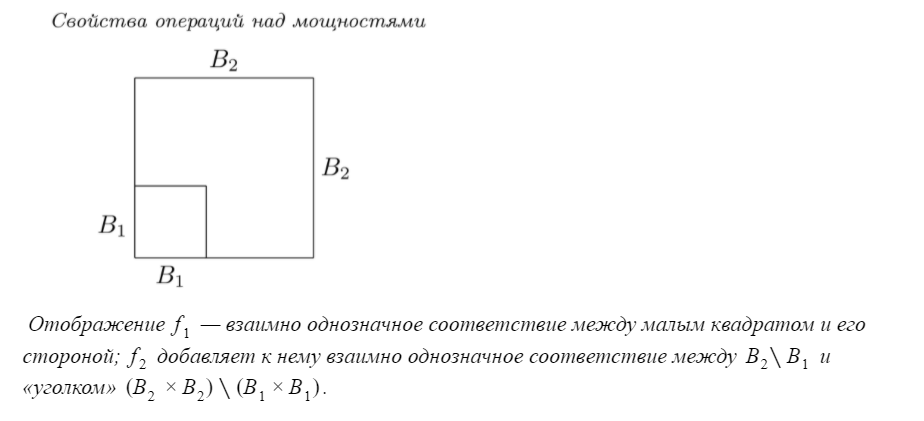
\includegraphics[width=14cm]{images/2.12 1.png}
\end{center}

Теперь применим лемму Цорна. Для этого нужно убедиться, что любое линейно упорядоченное (в смысле описанного порядка) множество пар указанного вида имеет верхнюю границу. В самом деле, объединим все первые компоненты этих пар; пусть $B$ — их объединение. Как обычно, согласованность отображений (гарантируемая определением порядка) позволяет соединить отображения в одно. Это отображение (назовём его $f$) отображает $B$ в $B \times B$. Оно будет инъекцией: значения $f(b')$ и $f(b'')$ при различных $b'$ и $b''$ различны (возьмем большее из множеств, которым принадлежат $b'$ и $b''$; на нём $f$ является инъекцией по предположению). С другой стороны, $f$ является сюръекцией: для любой пары $(b', b'') \in B \times B$ возьмём множества, из которых произошли $b'$ и $b''$, выберем из них большее и вспомним, что мы имели взаимно однозначное соответствие между ним и его квадратом.

По лемме Цорна в нашем частично упорядоченном множестве существует максимальный элемент. Пусть этот элемент есть $(B, f)$. Мы знаем, что $f$ есть взаимно однозначное соответствие между $B$ и $B \times B$ и потому $|B| = |B| \times |B|$. Теперь есть две возможности. Если $B$ равномощно $A$, то $B \times B$ равномощно $A \times A$ и всё доказано. Осталось рассмотреть случай, когда $B$ не равномощно $A$, то есть имеет меньшую мощность (большей оно иметь не может, будучи подмножеством). Пусть $C$ -- оставшаяся часть $A$, то есть $A \backslash B$.

Тогда $|A| = |B| + |C| = max(|B|, |C|)$, следовательно, $C$ равномощно $A$ и больше $B$ по мощности. Возьмём в $C$ часть $C'$, равномощную $B$, и положим $B' = B + C'$.

\begin{center}
    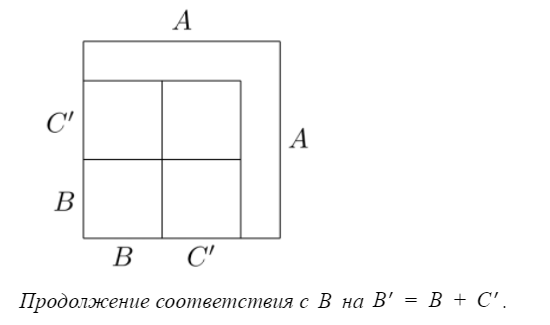
\includegraphics[width=7.5cm]{images/2.12 2.png}
\end{center}

Обе части множества $B'$ равномощны $B$. Поэтому $B' \times B'$ разбивается на $4$ части, каждая из которых равномощна $B \times B$, и, следовательно, равномощна B (т.к. $C', (B' \times B'), (B \times B)$  равномощны $B$). В итоге мы получаем большую пару $(B', f')$, что противоречит утверждению леммы Цорна о максимальности. Таким образом, этот случай невозможен.

    \newpage
    \section{№3 Изоморфизм группы}

\begin{reminder}
  наименьшее k --- порядок группы, если $g ^ k = e$.
\end{reminder}

\begin{note}
  $(Z_n, +) \quad \ord a = \frac{n}{\gcdru(a, n)}$
  \[S_n \ord \Pi = \gcdru(\text{\#len}).\] Где \#len --- длинна циклов.
\end{note}

\subsection{Порядки перестановки}

\begin{reminder}
  $\Pi: (a_0, a_1, \dots, a_{l - 1})$. Если $\Pi ^ {s} = \id \Ra \Pi ^{s} (a_0) = a_0 \Ra l \mid s$
  \[\ord \Pi = l.\]
\end{reminder}

\begin{example}
  $\pi = \underbrace{(\dots)}_{l_1}\underbrace{(\dots)}_{l_2}\underbrace{(\dots)}_{l_3} \dots \underbrace{(\dots)}_{l_s}$. Тогда имеем $\ord \pi = \gcdru(l_1, \dots, l_s).$
\end{example}

\begin{example}
  $\mid G \mid = n, \ d = 80, \ \mid S_{12} \mid = 12!$
  \[\gcdru(l_1, \dots, l_s) = 80, \]
  \[l_1 + \dots + l_s = 12.\]
  То есть невозможно.
\end{example}

\subsection{Основная теорема арифметики}
\begin{theorem}[Основная теорема арифметики]
  Для любого n > 1 --- \ul{однозачно} представялется произведением простых множителей (с точностью до пересестановки множителей).
\end{theorem}

\begin{example}
  $80 = 2 ^ 4 \cdot 5 = 2 ^ 2 \cdot 5 \cdot 2 ^ 2$.
\end{example}

\begin{proof}
  По индукции. $n = 2$ --- база. Пусть < n --- существует.
  \begin{enumerate}
    \item[(1)] n --- простое,
    \item[(2)] $n = ab, \ 1 < a, b < n$.
  \end{enumerate}
  Пусть $x \not \equiv 0 \mod p \Ra x^{-1} \cdot x \equiv 1 \mod p \Ra y \equiv 0 \mod (p)$.
\end{proof}

\begin{lemma}
  p --- простое, то есть $xy \equiv 0 \mod (p) \Ra$
  \[x \equiv 0 \mod (p) \vee y \equiv 0 \mod (p).\]
\end{lemma}

\begin{proof}
  $\underbrace{p_1 \dots p_k}_{\text{Делится на } p_1} = q_1 \dots q_s$, где $p_i, q_j$ --- простое. Тогда утверждается, что $p_i \not = q_i$ --- в силу закона сокращения.
  \[\Ra p_1 \mid q_k \Ra p_1 = q_k.\] В силу того, что левая часть делится на $p_1$.
\end{proof}

\begin{proposition}
  $n = p_1^{a_1} \dots p_t^{a_t} \dots, \quad p_1 < p_2 < p_3 < \dots < p_t < \dots$
  \[p_k \nmid n \Ra a_k = 0.\]
\end{proposition}

\begin{example}
  \[x = p_1^{a_1} \dots p_t^{a_t} \dots ,\]
  \[y = p_1^{b_1} \dots p_t^{b_t} \dots ,\]
  \[x \mid y \Lra a_i \leq b_i,\]
  \[\gcdru(x, y) = p_1^{\min (a_1, b_1)} \cdot \ldots \cdot p_t^{\min (a_t, b_t) },\]
  \[\lcm(x, y) = p_1^{\max (a_1, b_1)} \cdot \ldots \cdot p_t^{\max (a_t, b_t) }.\]
\end{example}

\subsection{Класс групп}
\begin{definition}
  Группа G --- циклическая, если:
  \[G = \langle g \rangle.\]
  Обозначение: $C_n$ --- циклическая.
\end{definition}

\begin{corollary}
  Любая циклическая группа --- абелева. То есть, для любого элемента выполнено: $g^{i + j} = g^i \cdot g^j$.
\end{corollary}

\begin{example}
  $| (Z_{\delta}^{\text{*}}, \cdot) | = 4, \quad 1^2 \equiv 3^2 \equiv 5^2 \equiv 7^2 \equiv 1 \mod \delta$.
\end{example}

\begin{theorem}
  Если, $G = \{ g^i, i \in \ZZ \} = \langle g \rangle$, то изоморфны и $(\ZZ, +)$ и $(Z_n, +)$.
\end{theorem}

\begin{example}
  $|G| = \infty$ --- все степени различны.
  \[g^i = g ^ j \Lra g^{j - i} = e,\]
  \[k \raone g^k,\]
  \[(\ZZ, +) \ra G,\]
  \[g^{n + qn} = g^i \cdot g^{qn} = g^i \cdot (g^n)^q.\]
\end{example}

\begin{theorem}
  Подгруппа циклической группы --- циклическая.
\end{theorem}

\begin{example}
  Пусть $G < (\ZZ, +)$, тогда 
  \[\quad d = \min (x: x > 0 \quad x \in G), \]
  \[g \in G \quad g = qd + r, \ 0 \leq d, \]
  \[t = g - qd \in G \Ra r = 0.\]
  Если $G < (Z_n, +)$, тогда
  \[d  = \min (x: 0 < x < n \quad [x] \in G),\]
  \[d \mid n \quad n = qd + r \Ra r \in G \Ra r = 0.\]
\end{example}

\subsection{Изоморфизм групп}
\begin{example}[1]
  $(Z_6, +)$. Нейтальный --- $0$. Кратные элементы --- $ka$.
\end{example}

\begin{example}[2]
  $g = \langle(12)(345)\rangle, \quad \ord g = 6$
\end{example}

\begin{definition}
  Изоморфизм групп, это отображение, такое что:
  \[\phi : G_1 \ra G_2\]
  \begin{enumerate}
    \item[(1)] $\phi$ --- биекция,
    \item[(2)] $\phi(xy) = \phi(x) \ \phi(y)$. Для любых $x, y \in G$.
  \end{enumerate}
  Обозначение: $G_1 \cong G_2$.
\end{definition}

\begin{note}
  Тогда имеем, что примеры (1) и (2) --- изоморфны.  
\end{note}

\subsection{Прямое произведение групп}
\begin{definition}
  Пусть G, H --- группы. Тогда, $G \times H = \{(g, h): g \in G, h \in H\}$. Тогда имеем несколько свойств: 
  
  \begin{enumerate}
    \item $(g_1, h_1) \cdot (g_2, h_2) = (g_1 \cdot g_2, h_1 \cdot h_2)$,
    \item $\ord (g, h) = \lcm(\ord g, \ord h)$,
    \item $(g, h)^k = (g^k, h^k) = (e, e)$.
  \end{enumerate}
\end{definition}

\begin{proposition}
  $\gcdru(p, q ) = 1$, тогда имеем: $C_p \times C_q \cong C_{pq}$.
\end{proposition}

\begin{proof}
  $\ord(1, 1) = \gcdru(p, q) = \frac{pq}{1} = pq = |C_p \times C_q|$.
\end{proof}

\begin{corollary}
  $C_p \times C_q \text{--- циклическая} \cong C_{pq}$.
\end{corollary}

\subsection{Мультипликативность функции Эйлера}

\begin{proposition}
  % $\gcdru(p, q) = 1 \Ra \underbrace{\phi(pq)}_{\text{Число порождающих в } C_{pq}} = \underbrace{\phi(p) \phi (q)}_{\text{Число порождающих в } C_p \times C_q}$
  Если $\gcdru(p, q) = 1$, то выполено равенство:
  \[\phi(pq) = \phi(p) \phi (q).\]

  % $\phi(n) = |(Z_n^{\text{*}}, \cdot)|$
\end{proposition}

\begin{proof}
  Равенство верное, в силу того, что левая часть --- число порождающих в $C_{pq}$, а справа --- число порождающих в $C_p \times C_q$.
\end{proof}

\begin{proposition}
  Количество пораждающих в $C_n$ равно $\phi(n)$.
\end{proposition}

\begin{proof}
  \[(x, y) \in C_p \times C_q, \]
  \[\ord (x, y) = \gcdru(\ord x, \ord y) = pq \Ra \ord x = p, \quad \ord y = q.\]    
\end{proof}

\begin{example}
  Пусть $n = p_1^{q_1} \dots p_t^{a_t}, \quad a_i > 0$, тогда

  \[\phi (p^n) = p^n - p^{n - 1}.\]В силу того, что $x \not \equiv 0 \mod (p^n) \Lra x \equiv 0 \mod (p)$.

  \[\phi(n) = (p_t^{a_t} - p_t^{a_t - 1}) = n (1 - \frac{1}{p_1}) (1 - \frac{1}{p_2}) \dots (1 - \frac{1}{p_t}).\]
\end{example}



    \newpage
    \subsection{Ориентация на плоскости и в пространстве. Ориентированные площадь и объем (смешанное произведение). Свойства ориентированных площади и объема. Выражение ориентированных площади и объема в произвольном базисе.}
    
    \begin{definition}
    	Пусть плоскость $P_2$ вложена в пространство $P_3$, и выделено одно из полупространств в $P_3$ относительно этой плоскости. Базис $(\overline{a}, \overline{b})$ в $V_2$ называется \textit{положительно ориентированным}, если поворот на кратчайший угол, который переводит вектор $\overline{a}$ в вектор $\overline{a'} \parallel \overline{b}$, происходит против часовой стрелки при взгляде из выделенного полупространства. В противном случае базис называется \textit{отрицательно ориентированным}.
    \end{definition}
    
    \begin{note}
    	Базисы $(\overline{a}, \overline{b})$ и $(\overline{b}, \overline{a})$ всегда ориентированы по-разному.
    \end{note}
    
    \begin{definition}
    	Базис $(\overline{a}, \overline{b}, \overline{c})$ в $V_3$ называется \textit{правой тройкой}, если базис $(\overline{a}, \overline{b})$ в плоскости $V_2$, содержащей эти два вектора, ориентирован положительно относительно полупространства, содержащего вектор $\overline{c}$, отложенный от точки в $P_2$. В противном случае базис называется \textit{левой тройкой}.
    \end{definition}
    
    \begin{proposition}~
    	\begin{enumerate}
    		\item Базисы $(\overline{a}, \overline{b}, \overline{c})$ и $(\overline{b}, \overline{a}, \overline{c})$ в $V_3$ всегда ориентированы по-разному.
    		\item Базисы $(\overline{a}, \overline{b}, \overline{c})$ и $(\overline{a}, \overline{c}, \overline{b})$ в $V_3$ всегда ориентированы по-разному.
    	\end{enumerate}
    \end{proposition}
    
    \begin{proof}~
    	\begin{enumerate}
    		\item Так как базисы $(\overline{a}, \overline{b})$ и $(\overline{b}, \overline{a})$ ориентированы по-разному, то базисы $(\overline{a}, \overline{b}, \overline{c})$ и $(\overline{b}, \overline{a}, \overline{c})$ тоже ориентированы по-разному.
    		\item Пусть $\overline{OA} = \overline{a}$, $\overline{OB} = \overline{b}$, $\overline{OC} = \overline{c}$. Будем поворачивать направленный отрезок $\overline{OC}$ в плоскости $(BOC)$, пока он не перейдет в такой направленный отрезок $\overline{OC'}$, что $C$ и $C'$ лежат по разные стороны от $OB$. Ориентация базиса $(\overline{a}, \overline{b}, \overline{c'})$ противоположна ориентации $(\overline{a}, \overline{b}, \overline{c})$, но совпадает с ориентацией $(\overline{a}, \overline{c}, \overline{b})$.\qedhere
    	\end{enumerate}
    \end{proof}
    
    \begin{note}
    	В силу утверждения выше, всевозможные перестановки базиса $(\overline{a}, \overline{b}, \overline{c})$ делятся на два класса противоположной ориентации:
    	\begin{itemize}
    		\item $(\overline{a}, \overline{b}, \overline{c})$, $(\overline{c}, \overline{a}, \overline{b})$ и $(\overline{b}, \overline{c}, \overline{a})$
    		\item $(\overline{b}, \overline{a}, \overline{c})$, $(\overline{c}, \overline{b}, \overline{a})$ и $(\overline{a}, \overline{c}, \overline{b})$
    	\end{itemize}
    \end{note}
    
    \begin{definition}
    	Пусть $\overline{a}, \overline{b} \in V_2$, и в плоскости $V_2$ задана ориентация. \textit{Ориентированной площадью} $S(\overline{a}, \overline{b})$ называется площадь параллелограмма, построенного на этих векторах, взятая со знаком, соответствующим ориентации $(\overline{a}, \overline{b})$.
    \end{definition}
    
    \begin{definition}
    	Пусть $\overline{a}, \overline{b}, \overline{c} \in V_3$. \textit{Ориентированным объемом} $V(\overline{a}, \overline{b}, \overline{c})$ называется объем параллелепипеда, построенного на этих векторах, взятая со знаком, соответствующим ориентации $(\overline{a}, \overline{b}, \overline{c})$. Эта величина также называется \textit{смешанным произведением} векторов $\overline{a}, \overline{b}, \overline{c}$ и обозначается через $(\overline{a}, \overline{b}, \overline{c})$.
    \end{definition}
    
    \begin{note}
    	Определения выше корректны, поскольку в них не требуется определять ориентацию набора векторов, не являющегося базисом:
    	\begin{enumerate}
    		\item $S(\overline{a}, \overline{b}) = 0$ $\Leftrightarrow$ $\overline{a}$ и $\overline{b}$ коллинеарны.
    		\item $V(\overline{a}, \overline{b}, \overline{c}) = 0$ $\Leftrightarrow$ $\overline{a}$, $\overline{b}$ и $\overline{c}$ компланарны.
    	\end{enumerate}
    \end{note}
    
    \begin{proposition}~
    	\begin{enumerate}
    		\item Если базис $e = (\overline{e_1}, \overline{e_2})$ в $V_2$ "--- ортонормированный, то $S(\overline{e_1}, \overline{e_2}) = \pm 1$.
    		\item Если базис $e = (\overline{e_1}, \overline{e_2}, \overline{e_3})$ в $V_3$ "--- ортонормированный, то $V(\overline{e_1}, \overline{e_2}, \overline{e_3}) = \pm 1$.
    	\end{enumerate}
    \end{proposition}
    
    \begin{proof}~
    	\begin{enumerate}
    		\item Параллелограмм, образованный векторами $\overline{e_1}$ и $\overline{e_2}$, "--- это квадрат со стороной $1$, поэтому $|S(\overline{e_1}, \overline{e_2})| = 1$.
    		\item Параллелепипед, образованный векторами $\overline{e_1}$, $\overline{e_2}$ и $\overline{e_3}$, "--- это куб со стороной $1$, поэтому $|V(\overline{e_1}, \overline{e_2}, \overline{e_3})| = 1$.\qedhere
    	\end{enumerate}
    \end{proof}

    \begin{theorem}
    	Ориентированный объем обладает следующими свойствами:
    	\begin{enumerate}
    		\item $\forall \overline{a}, \overline{b}, \overline{c} \in V_n: V(\overline{a}, \overline{b}, \overline{c}) = -V(\overline{b}, \overline{a}, \overline{c}) = -V(\overline{a}, \overline{c}, \overline{b})$ (кососимметричность)
    		\item $\forall \overline{a_1}, \overline{a_2}, \overline{b}, \overline{c} \in V_n: V(\overline{a}, \overline{b}, \overline{c_1} + \overline{c_2}) = V(\overline{a}, \overline{b}, \overline{c_1}) + V(\overline{a}, \overline{b}, \overline{c_2})$
    		
    		$\forall \lambda \in \R: \forall \overline a, \overline b, \overline c \nolinebreak\in\nolinebreak V_n \nolinebreak: \nolinebreak V(\overline{a}, \overline{b}, \lambda\overline{c}) \hm= \lambda V(\overline{a}, \overline{b}, \overline{c})$ (линейность по третьему аргументу)
    	\end{enumerate}
    \end{theorem}
    
    \begin{proof}~
    	\begin{enumerate}
    		\item Если $\overline{a}$, $\overline{b}$ и $\overline{c}$ компланарны, то утверждение очевидно. Иначе --- объем параллепипеда при перестановке векторов базиса не меняется по модулю, но меняет знак при смене ориентации.
    		\item Если $\overline{a}$ и $\overline{b}$ коллинеарны, то утверждение очевидно. Пусть теперь это не так, тогда рассмотрим направленные отрезки $\overline{OA} = \overline{a}$, $\overline{OB} = \overline{b}$, $\overline{OC} = \overline{c}$. Обозначим через $\overline d$ вектор такой, что $|\overline{d}| = 1$, $\overline{d} \perp (AOB)$ и $(\overline{a}, \overline{b}, \overline{d})$ "--- правая тройка, и пусть $\overline{OD} = \overline{d}$.
    		
    		Заметим теперь, что $\forall \overline{c} \in V_n: V(\overline{a}, \overline{b}, \overline{c}) = |S(\overline{a}, \overline{b})|(\overline{c}, \overline{d})$, поскольку выполнены равенства $(\overline{c}, \overline{d}) = (\pr_{\overline{d}}\overline{c}, \overline{d}) \hm{=} \pm |\pr_{\overline{d}}\overline{c}| = \pm h$, где $h$ "--- высота параллелепипеда, а знак соответствует ориентации базиса $(\overline{a}, \overline{b}, \overline{c})$. Тогда линейность ориентированного объема следует из линейности скалярного произведения.\qedhere
    	\end{enumerate}
    \end{proof}
    
    \begin{theorem}
    	Пусть $e = (\overline{e_1}, \overline{e_2})$ "--- базис в $V_2$, $\overline{a}, \overline{b} \hm{\in} V_2$, $\overline{a} \leftrightarrow_{e} \alpha$, $\overline{b} \leftrightarrow_{e} \beta$. Тогда верно следующее равенство:
    	\[S(\overline{a}, \overline{b}) = \begin{vmatrix}
    	\alpha_1 & \beta_1\\
    	\alpha_2 & \beta_2
    	\end{vmatrix}S(\overline{e_1}, \overline{e_2})\]
    \end{theorem}
    
    \begin{proof}
    	В силу линейности ориентированной площади, имеем:
    	\[S(\overline{a}, \overline{b}) = S\left(\sum_{i = 1}^{2} \alpha_i\overline{e_i}, \sum_{j = 1}^{2} \beta_j\overline{e_j}\right) = \sum_{i = 1}^{2} \sum_{j = 1}^{2}\alpha_i\beta_jS(\overline{e_i}, \overline{e_j})\]
    	
    	Поскольку для любого $i \in \{1, 2\}$ выполнено $S(\overline{e_i}, \overline{e_i}) = 0$, то:
    	\[S(\overline{a}, \overline{b}) = \begin{vmatrix}
    	\alpha_1 & \beta_1\\
    	\alpha_2 & \beta_2
    	\end{vmatrix}S(\overline{e_1}, \overline{e_2})\]
    	
    	Получено требуемое.
    \end{proof}
    
    \begin{theorem}
    	Пусть $e = (\overline{e_1}, \overline{e_2}, \overline{e_3})$ "--- базис в $V_3$, $\overline{a}, \overline{b}, \overline{c} \hm{\in} V_3$, $\overline{a} \leftrightarrow_{e} \alpha$, $\overline{b} \leftrightarrow_{e} \beta$, $\overline{c} \leftrightarrow_{e} \gamma$. Тогда верно следующее равенство:
    	\[V(\overline{a}, \overline{b}, \overline{c}) = \begin{vmatrix}
    	\alpha_1 & \beta_1 & \gamma_1\\
    	\alpha_2 & \beta_2 & \gamma_2\\
    	\alpha_3 & \beta_3 & \gamma_3
    	\end{vmatrix}V(\overline{e_1}, \overline{e_2}, \overline{e_3})\]
    \end{theorem}
    
    \begin{proof}
    	В силу линейности ориентированного объема, имеем:
    	\[V(\overline{a}, \overline{b}, \overline{c}) = V\left(\sum_{i = 1}^{3} \alpha_i\overline{e_i}, \sum_{j = 1}^{3} \beta_j\overline{e_j},  \sum_{k = 1}^{3} \gamma_k\overline{e_k}\right) = \sum_{i = 1}^{3} \sum_{j = 1}^{3}\sum_{k = 1}^{3}\alpha_i\beta_j\gamma_kV(\overline{e_i}, \overline{e_j}, \overline{e_k})\]
    	
    	Поскольку для любых $i, j, k \in \{1, 2, 3\}$ таких, что $i = j$, $i = k$ или $j = k$, выполнено $V(\overline{e_i}, \overline{e_j}, \overline{e_k}) = 0$, то:
    	\[V(\overline{a}, \overline{b}, \overline{c}) = \begin{vmatrix}
    	\alpha_1 & \beta_1 & \gamma_1\\
    	\alpha_2 & \beta_2 & \gamma_2\\
    	\alpha_3 & \beta_3 & \gamma_3
    	\end{vmatrix}V(\overline{e_1}, \overline{e_2}, \overline{e_3})\]
    
    	Получено требуемое.
    \end{proof}
    
    \begin{note}
    	Из теорем выше следуют, в частности, такие свойства:
    	\begin{itemize}
    		\item Если $e$ "--- положительно ориентированный ортонормированный базис в $V_2$, то для любых $\overline a, \overline b \in V_2$ таких, что $\overline a \leftrightarrow_e \alpha$ и $\overline b \leftrightarrow_e \beta$, верно равенство $S(\overline{a}, \overline{b}) = |\alpha\beta|$.
    		\item Если $e$ "--- правый ортонормированный базис в $V_3$, то для любых $\overline a, \overline b, \overline c \in V_3$ таких, что $\overline a \leftrightarrow_e \alpha$, $\overline b \leftrightarrow_e \beta$ и $\overline c \leftrightarrow_e \gamma$, верно равенство $V(\overline{a}, \overline{b}, \overline{c}) \hm{=} |\alpha\beta\gamma|$.
    		\item Если $e$ "--- базис в $V_2$, $\overline a, \overline b \in V_2$, $\overline a \leftrightarrow_e \alpha$, $\overline b \leftrightarrow_e \beta$, то векторы $\overline{a}$ и $\overline{b}$ коллинеарны $\Leftrightarrow$ $|\alpha\beta| = 0$.
    		\item Если $e$ "--- базис в $V_3$, $\overline a, \overline b, \overline c \in V_3$, $\overline a \leftrightarrow_e \alpha$, $\overline b \leftrightarrow_e \beta$, $\overline c \leftrightarrow_e \gamma$, то векторы $\overline{a}$, $\overline{b}$ и $\overline{c}$ компланарны $\Leftrightarrow$ $|\alpha\beta\gamma| = 0$.
    	\end{itemize}
    \end{note}
    

    \newpage
    \section{5. Непрерывность функции в точке. Равносильные определения непрерывности. Теорема о непрерывности композиции. Точки разрыва, их классификация. Теорема о разрывах монотонной функции.}
    %\overset{o}{B_{\delta}}
    \begin{definition}
        Пусть $E \subset \R$, задана функция $f: E \to \R$ и $a \in E$. Функция $f$ называется \textit{непрерывной} в точке $a$, если
        \[\forall \epsilon > 0 \ \exists \delta > 0 \ \forall x \in E \ (x \in B_{\delta}(a) \Rightarrow f(x) \in B_{\epsilon}(f(a)))\]
    \end{definition}

    \begin{theorem}
        Пусть $f: E \to \R$, $a \in E$. Следующие условия эквивалентны:
        \begin{enumerate}
            \item функция $f$ непрерывна в точке $a$;
            \item $\forall \{x_{n}\}$, $x_{n} \in E \ (x_{n} \to a \Rightarrow f(x_{n}) \to f(a))$;
            \item $a$ -- изолированная точка множества $E$, или $a$ -- предельная точка $E$ и $\lim_{x \to a} f(x) = f(a)$.
        \end{enumerate}
    \end{theorem}

    \begin{proof} \ \\
        (1) $\Rightarrow$ (2) Рассмотрим произвольную последовательность точек $x_{n} \in E$, сходящуюся к $a$. Покажем, что $f(x_{n}) \to f(a)$. Зафиксируем $\epsilon > 0$. По определению непрерывности найдется такое $\delta > 0$, что $|f(x) - f(a)| < \epsilon$ для всех $x \in B_{\delta}(a) \cap E$. Так как $x_{n} \to a$, то существует такой номер $N$, что $x_{n} \in B_{\delta}(a) \cap E$ при всех $n \geq N$ и, значит, $|f(x_{n}) - f(a)| < \epsilon$ при всех $n \geq N$. \\
        (2) $\Rightarrow$ (3) Если $a$ -- предельная точка $E$, то в силу (2) $\lim_{x \to a} f(x) = f(a)$ по определению Гейне предела функции. Если $a$ не является предельной точкой $E$, то по определению $a$ -- изолированная точка $E$. \\
        (3) $\Rightarrow$ (1) Если $a$ изолирована, то $B_{\delta_{0}}(a) \cap E = \{a\}$ для некоторого $\delta_{0} > 0$. Тогда определение непрерывности в точке $a$ выполняется для $\delta = \delta_{0}$. Пусть $a$ предельная точка $E$. По определению Коши предела функции $\forall \epsilon > 0 \ \exists \delta > 0 \ \forall x \in E \ (0 < |x - a| < \delta \Rightarrow |f(x) - f(a)| < \epsilon)$. Но последняя импликация очевидно выполняется и для $x = a$. Значит, функция $f$ непрерывна в точке $a$.
    \end{proof}

    \begin{theorem}{О непрерывности композиции}\\
        Пусть $f: E \to \R$, и $g: D \to \R$, причем $f(E) \subset D$. Если функция $f$ непрерывна в точке $a$, функция $g$ непрерывна в точке $f(a)$, то композиция $g \circ f: E \to \R$ непрерывна в точке $a$.
    \end{theorem}

    \begin{proof}
        Пусть $x_{n} \in E$ и $x_{n} \to a$. Тогда $f(x_{n}) \to f(a)$ в силу непрерывности $f$ в точке $a$, и $g(f(x_{n})) \to g(f(a))$ в силу непрерывности $g$ в точке $f(a)$. По теореме об эквивалентных определениях непрерывности, функция $g\circ f$ непрерывна в точке $a$.
    \end{proof}

    \begin{definition}
        Пусть $f: E \to \R$, $a \in E$. Если $f$ не является непрерывной в точке $a$, то говорят, что $f$ \textit{разрывна} в точке $a$, а точку $a$ называют \textit{точкой разрыва} функции $f$. 
    \end{definition}

    Пусть функция задана в проколотой окрестности точки $a$. Если существуют конечные пределы $f(a - 0)$ и $f(a + 0)$, но не все числа $f(a - 0)$, $f(a + 0)$ и $f(a)$ равны между собой (случай, когда $f$ не определена в самой точке $a$ тоже допускается), то $a$ называется \textit{точкой разрыва ${\MakeUppercase{\romannumeral 1}}$ рода}. В противном случае, т.е. хотя бы один из односторонних пределов бесконечен или не существует, то $a$ называется \textit{точкой разрыва ${\MakeUppercase{\romannumeral 2}}$ рода} $f$.\\
    Если $a$ -- точка разрыва ${\MakeUppercase{\romannumeral 1}}$ рода и $f(a - 0) = f(a + 0)$, то $a$ называется \textit{точкой устранимого разрыва} функции $f$.

    \begin{theorem}{О разрывах монотонной функции}\\
        Если функция $f$ монотонна на конечном или бесконечном интервале $(a, b)$, то $f$ может иметь на $(a, b)$ разрывы только ${\MakeUppercase{\romannumeral 1}}$ рода, причем их не более чем счетное множество.
    \end{theorem}

    \begin{proof}
        Пусть для определенности $f$ нестрого возрастает. По следствию из теоремы об односторонних пределах монотонной функции, для любой точки $c \in (a, b)$ существуют конечные $f(c + 0)$ и $f(c - 0)$, причем $f(c - 0) \leq f(c) \leq f(c + 0)$. Поэтому, если $f$ разрывна в точке $c$, то $f(c - 0) < f(c + 0)$ и, значит, $c$ -- точка разрыва ${\MakeUppercase{\romannumeral 1}}$ рода.\\
        Пусть $c, d \in (a, b)$, причем $c < d$. Ввиду возрастания функции $\inf_{(c, b)}f(x) = \inf_{(c, d)}f(x)$ и $\sup_{(a, d)}f(x) = \sup_{(c, d)}f(x)$ и, значит,
        \[f(c + 0) = \inf_{x \in (c, d)} f(x) \leq \sup_{x \in (c, d)} f(x) = f(d - 0).\]
        Поэтому, если $c, d$ -- точки разрыва $f$, то интервалы $(f(c - 0), f(c + 0))$ и $(f(d - 0), f(d + 0))$ не пересекаются. Поставим в соответствие каждому такому интервалу рациональное число, содержащееся в нем. Тем самым установим биекцию между множеством таких интервалов и подмножеством $\Q$. Любое подмножество $\Q$ не более чем счетно, поэтому множество точек разрыва $f$ не более чем счетно.
    \end{proof}

    \newpage
    \subsection{Прямая на плоскости, различные способы задания, их эквивалентность. Формула для расстояния от точки до прямой в прямоугольной системе координат. Условия пересечения и параллельности двух прямых. Пучок прямых.}
    
    \begin{definition}
    	\textit{Направляющим вектором} прямой $l \subset P_3$ называется вектор $\overline{a} \in V_3$, $\overline{a} \ne \overline 0$, представителем которого является направленный отрезок, лежащий в $l$.
    \end{definition}
    
    \begin{definition}
    	Пусть $l \subset P_2$ "--- прямая с направляющим вектором $\overline{a} \in V_2$, $M \in l$, и в декартовой системе координат $(O, e)$ в $P_2$ выполнены соотношения $\overline{a} \leftrightarrow_{e} (\alpha_1, \alpha_2)^T$, $M \leftrightarrow_{(O, e)} (x_0, y_0)^T$, $\overline{r_0} := \overline{OM}$.
    	\begin{itemize}
    		\item \textit{Векторно-параметрическим уравнением прямой} называется следующее семейство уравнений:
    		\[\overline{r} = \overline{r_0} + t\overline{a},~t \in \mathbb{R}\]
    		\item \textit{Параметрическим уравнением прямой} называется следующее семейство систем:
    		\[\left\{
    		\begin{aligned}
    			x = x_0 + t\alpha_1\\
    			y = y_0 + t\alpha_2
    		\end{aligned}
    		\right.,~t \in \R
    		\]
    		\item \textit{Каноническим уравнением прямой} называется следующее уравнение:
    		\[\frac{x - x_0}{\alpha_1} = \frac{y - y_0}{\alpha_2}\]
    	\end{itemize}
    \end{definition}
    
    \begin{note}
    	Множество точек $X \in P_2$ таких, что $X \leftrightarrow_{(O, e)} (x, y)^T$, $\overline{r} := \overline{OX}$, являющихся решениями любого из уравнений прямой выше, совпадает с прямой $l$. Действительно, $X \in l \lra MX \parallel l \lra \overline{MX} \parallel \overline{a}$.
    \end{note}
    
    \begin{note}
    	В случае канонического уравнения прямой, если без ограничения общности $\alpha_1 = 0$, то тогда $\alpha_2 \ne 0$, и следует считать, что исходное уравнение эквивалентно условию $x = x_0$. Отметим также, что каноническое уравнение прямой эквивалентно следующему такому уравнению:
    	\[\alpha_2 x - \alpha_1 y + (\alpha_1 y_0 - \alpha_2 x_0) = 0\]
    \end{note}
    
    \begin{definition}
    	Пусть $A, B, C \in \R$, $A^2+B^2 \ne 0$. \textit{Общим уравнением прямой} называется следующее уравнение:
    	\[Ax+By+C = 0\]
    \end{definition}
    
    \begin{theorem}
        Пусть $l_{1}: A_{1}x + B_{1}y + C_{1} = 0$, $l_{2}: A_{2}x + B_{2}y + C_{2} = 0$. 
        \begin{enumerate}
            \item $l_1 \times l_2 \lra \begin{vmatrix}
                A_1 & B_1 \\
                A_2 & B_2
            \end{vmatrix} \neq 0;$
            \item $l_1 \parallel l_2 \lra \begin{vmatrix}
                A_1 & B_1 \\
                A_2 & B_2
            \end{vmatrix} = 0;$
            \item $l_1 = l_2 \lra$ их уравнения пропорциональны.
        \end{enumerate}
    \end{theorem}
    
    \begin{proof}
        1. Следует из п.2;\\
        2. Нормальные векторы прямых $l_1$ и $l_2$ имеют координаты $(A_1,B_1)$ и $(A_2, B_2)$ соответственно, а условие параллельности прямых запишется как $\begin{cases}
            A_1 = t A_2\\
            B_1 = t B_2
        \end{cases}$, откуда и следует искомое.\\
        3. Пусть $l_1 = l_2$. Тогда $\begin{cases}
            A_2 = \lambda A_1\\
            B_2 = \lambda B_1
        \end{cases}$. Запишем уравнения прямых $l_1: A_{1}x + B_{1}y + C_1 = 0$, $l_2: \lambda(A_{1}x + B_{1}y) + C_2 = 0$. В частности, для общего решения $(x_{0}, y_{0})$ имеем: $A_{1}x_{0} + B_{1}y_{0} + C_1 = 0$, $\lambda(A_{1}x_{0} + B_{1}y_{0}) + C_2 = 0$. Домножим первое равенство на $(-1)$ и прибавим ко второму, получим $C_2 - \lambda C_1 = 0$, $C_2 = \lambda C_1$.
        Заметим, что первые два пункта являются следствием теоремы Крамера.
    \end{proof}
    
    \begin{definition}
    	\textit{Вектором нормали} прямой $l \subset P_3$ называется вектор $\overline{n} \in V_3$, $\overline{n} \ne \overline 0$, представителем которого является направленный отрезок, ортогональный прямой $l$.
    \end{definition}
    
    \begin{definition}
    	Пусть $l \subset P_2$ "--- прямая с вектором нормали $\overline{n} \in V_2$, и пусть $M \in l$, $\overline{r_0} := \overline{OM}$. \textit{Нормальным уравнением прямой} называется следующее уравнение:
    	\[(\overline{r} - \overline{r_0}, \overline{n}) = 0\]
    \end{definition}
    
    \begin{note}
    	Множество точек $X \in P_2$, $\overline{r} := \overline{OX}$, являющихся решениями нормального уравнения прямой, совпадает с прямой $l$. Кроме того, это уравнение можно переписать в следующем виде при $\gamma := (\overline{r_0}, \overline{n})$:
    	\[(\overline{r}, \overline{n}) = \gamma\]
    \end{note}
    
    \begin{note}
    	Уравнения различного типа, задающие прямую, эквивалентны: из каждого из них можно получить любое другое.
    \end{note}
    
    \begin{definition}
    	\textit{Пучком прямых} называется либо множество всех прямых в $P_2$, проходящих через фиксированную точку $P \in P_2$, либо множество всех прямых, параллельных фиксированной прямой $l \subset P_2$.
    \end{definition}
    
    \begin{note}
    	Любые две прямые в $P_2$ лежат ровно в одном пучке.
    \end{note}
    
    \begin{theorem}
    	Пусть в декартовой системе координат $(O, e)$ в $P_2$ различные прямые $l_1, l_2$ заданы уравнениями $A_1x\hm{+}B_1y+C_1=0$, $A_2x+B_2y+C_2=0$. Тогда прямая $l \subset P_2$ лежит в одном пучке с прямыми $l_1$ и $l_2$ $\lra$ прямая $l$ задается уравнением следующего вида при некоторых $\alpha_1, \alpha_2 \in \R$:
    	\[\alpha_1(A_1x+B_1y+C_1) + \alpha_2(A_2x+B_2y+C_2) = 0\]
    \end{theorem}
    
    \begin{proof}~
    	\begin{itemize}
    		\item[$\la$] Возможны два случая:
    		\begin{enumerate}
    			\item Если $l_1 \cap l_2 = \{P\}$, $P \in P_2$, то координаты точки $P$ удовлетворяют требуемому уравнению, то есть $P \in l$.
    			\item Если $l_1 \parallel l_2$, то из требуемого уравнения направляющий вектор прямой $l$ параллелен направляющим векторам $l_1$ и $l_2$. В этом случае уравнение задает прямую не при всех $\alpha_1, \alpha_2 \in \R$, но если задает, то лежащую в данном пучке.
    		\end{enumerate}
    		
    		\item[$\ra$] Возможны два случая:
    		\begin{enumerate}
    			\item Если $l \cap l_1 \cap l_2 = \{P\}$, $P \in P_2$, то выберем на $l$ точку $Q \ne P$, $Q \leftrightarrow_{(O, e)} (x_0, y_0)^T$. Тогда $Q$ удовлетворяет уравнению с коэффициентами $\alpha_1 := A_2x_0+B_2y_0+C_2$, $\alpha_2 := -(A_1x_0+B_1y_0+C_1)$. Хотя бы один из коэффициентов ненулевой, поскольку $Q$ лежит не более, чем на одной из прямых $l_1$, $l_2$. Значит, такое уравнение задает $l$, так как ему удовлетворяют две различных точки этой прямой.
    			
    			\item Если $l \parallel l_1 \parallel l_2$, то аналогичным образом выберем любую точку $Q \in l$ и соответствующие коэффициенты, тогда полученное уравнение задает $l$ при условии, что оно задает прямую. Но оно всегда задает прямую, поскольку множество его решений непусто и не содержит хотя бы одну из прямых $l_1, l_2$.\qedhere
    		\end{enumerate}
    	\end{itemize}
    \end{proof}
    
    \begin{proposition}
    	Пусть в прямоугольной декартовой системе координат $(O, e)$ в $P_2$ прямая $l$ задана  уравнением $Ax\hm{+}By+C=0$, $M \in P_2$, $M \leftrightarrow_{(O, e)} (x_0, y_0)^T$. Тогда расстояние $\rho$ от точки $M$ до прямой $l$ равно следующей величине:
    	\[\rho = \frac{|Ax_0 + By_0 + C|}{\sqrt{A^2 + B^2}}\]
    \end{proposition}
    
    \begin{proof}
    	Пусть $\overline{n} \in V_2$, $\overline n \leftrightarrow_{e} (A, B)^T$ "--- вектор нормали прямой $l$, $\overline{r_0} := \overline{OM}$, и пусть $X \in l$, $\overline{r} := \overline{OX}$. Тогда:
    	\[\rho = |\pr_{\overline{n}}(\overline{r_0} - \overline{r})|
    	=
    	\left|\frac{(\overline{r_0} - \overline{r}, \overline{n})}{|\overline{n}|^2}\overline{n}\right|
    	=
    	\frac{|(\overline{r_0} - \overline{r}, \overline{n})|}{|\overline{n}|}
    	=
    	\frac{|Ax_0 + By_0 + C|}{\sqrt{A^2 + B^2}}\qedhere\]
    \end{proof}

    \newpage
    \section{№8 Кольца}

\subsection{Лемма Бернсайда}

\begin{lemma}
  Число орбит равно средней мощности стабилизатора элементов группы $G$.
  \[|X/G| = \frac{1}{G} \sum_{g \in G} |\stab g|\]
\end{lemma}

\begin{definition}
  Кольцо~--- множество с \underline{двумя} операциями: $(R, \cdot, +)$, такое что:
  \begin{enumerate}
    \item Является абелевой группой по сложению (0~--- нейтральный).
    \item Является ассоциативной по умножению (1~--- нейтральный).
    \item Двусторонняя дистрибутивность: 
    \begin{gather}
      a \cd (b + c) = a\cd + a \cd c \\
      (b + c) \cd a = b \cd a + c \cd a
    \end{gather}
  \end{enumerate}
\end{definition}

\begin{example}
  $\ZZ$, $\QQ$, $\RR$, $\Cm$.


  $2 \ZZ$~--- кольцо без $1$.

  % $M_n(\RR)$
  $\ZZ / n \ZZ$~--- вычеты по модулю $n$.
\end{example}

\begin{proposition}
  $a(b - c) = ab - ac, \quad (b-c)a = ba - ca$
\end{proposition}

\begin{proof}
  \begin{gather}
    a(b - c) + ac = a(b - c + c) = ab \\
    \Ra a(b - c) = ab - ac
  \end{gather}
\end{proof}

\begin{proposition}
  $0 \cd a = a \cd 0 = 0$.
\end{proposition}

\begin{proof}
  \[0 \cd a = (x - x) \cd a = xa - xa = 0\]
\end{proof}

\begin{proposition}
  Если в $\RR$ есть $1$, то $(-1) \cd (-1) = 1$.
\end{proposition}

\begin{proof}
  \[0 = (1 + (- 1)) \cd (-1) = 1 \cd (-1) + (-1) (-1) = (-1) + (-1) (-1)\]
  \[\Ra 1 = (-1) \cd (-1)\]
\end{proof}

\begin{note}
  Если по умножению группа, то:
  \[ 0 = 0^{-1} \cd 0 = 1 \Ra 0 = 1\]
  , то есть получаем, что: 
  \[\forall a: \ a = a \cd 1 = a \cd 0 = 0 \Ra |R| = 1\]  
\end{note}
В итоге, в кольце нельзя делить на ноль, тогда и только тогда, когда кольцо состоит из одного элемента (нуля). 

\begin{definition}
  Поле~--- множество вида: $(F, \cd, +)$, такое что:
  \begin{itemize}
    \item[$F1$]: Коммутативное кольцо с $1$ ($a \cd b = b \cd a$).
    \item[$F2$]: $0 \neq 1$.
    \item[$F3$]: $F^{*} = F \setminus  \{ 0 \}$~--- группа по умножению
  \end{itemize}
\end{definition}

\begin{example}
  $\FF = \ZZ / p \ZZ$~--- $p$ простое.
\end{example}

\begin{proposition}
  Если $n$~--- состовное, то $\ZZ / n \ZZ$~--- не поле.
\end{proposition}

\begin{proof}
  \begin{gather}
    [a]_n \cd [b]_n = [0]_n \\
    [a^{-1}]_n [a]_n [b]_n = [b]_n = [0]_n \\
    a^{-1} \cd a b = 0 \Ra b = 0
  \end{gather}
\end{proof}

\begin{definition}
  Делитель нуля:
  \[a \neq 0, \ b \neq 0, \ ab = 0 \]
\end{definition}

\begin{corollary}
  В кольцах есть делителя нуля, в полях нет.
\end{corollary}

\begin{example}
  Простые поля~--- $\FF_p, \ \QQ$.
\end{example}

\begin{lemma}
  В каждом поле есть простое подполе.
\end{lemma}

\begin{proof}
  Пусть $\{ n \cd 1 \} \subset F$~--- циклическая группа по сложению с образующей 1. 
  \[\{n, 1\} < \infty \Ra \deg F = p\]
  где $p$~--- простое. Тогда, кратные 1 - поле, то есть $\FF_p$.

  (Если $\{n \cd 1\} = + \infty$, то $\FF_p = \QQ$).
\end{proof}

    \newpage
    \section{9. Циклические подпространства. Теорема о нильпотентном операторе. Жорданова нормальная форма и жорданов базис линейного оператора. (Теорема существования жорданова базиса).}

\begin{definition}
    Оператор $\phi: V \to V$ называется \textit{нильпотентным}, если $\exists k \in \N :\: \phi^k = 0$. Наименьшее наутральное число $k$ такое, что $\phi^k = 0$, $\phi^{k-1} \neq 0$, называют \textit{индексом нильпотентности} относительно $\phi$. 
\end{definition}

\begin{definition}
    Пусть $\phi$ -- нильпотентный и $x \in V$ -- вектор, имеющий высоту $k$. 
    Рассмотрим $U = \langle x, \phi(x), \ldots, \phi^{k-1}(x)\rangle$.
    Построенное инвариантное подпространство $U$ называется \textit{циклическим подпространством}, 
    порожденным вектором $x$.
\end{definition}

\begin{theorem}[о нильпотентном операторе]~
    \label{th5.3}

    Пусть $\phi: V \to V$ -- нильпотентный оператор индекса нильпотентности $k$, $x \in V$ -- ненулевой вектор высоты $k$,
    $U = \langle x, \phi(x), \ldots, \phi^{k-1}(x) \rangle$ -- циклическое подпространство, инвариантное $\phi$.
    Тогда найдется $\phi$--инвариантное пространство $W$ дополнительное к $U$ такое, что $V = U \oplus W$.
\end{theorem}

\begin{proof}~

    \begin{enumerate}
        \item Пусть $W$ -- максимальное $\phi$-инвариантное подпространство в $V$, 
        такое что $U \cap W = {0}$. Предположим что $U + W < V$. 
        Тогда найдется ненулевой $a \in V$, такой что $ a \notin U + W$.  Пусть $l$ -- наименьшее 
        значение для которого $z = \phi^{l-1}(a) \notin W + U$, $\phi^l(a) \in W + U$. 
        Такое очевидно найдется так как $a \notin W + U$ и $\phi^{k}(a) = 0 \in W + U$.
        Таким образом в этом пункте мы нашли вектор $z \notin U+W$, такой что $\phi(z) \in U + W$.

        \item Пусть $\phi(z) = \displaystyle\sum_{s = 0}^{k-1} \alpha_s \phi^s(x) + w$, 
        при этом $\phi^s(x) \in U$, $w \in W$. Тогда:
        $$\phi^{k}(z) = \alpha_0 \phi^{k-1}(x) + 0 + \dots + 0 + \phi^{k-1}(w) = 0$$ 
        Тогда $\alpha_0 \phi^{k-1}(x) + \phi^{k-1}(w) = 0$. 
        В силу линейной независимости линейных подпространств 
        $\alpha_o \phi^{k-1}(x) = 0$, $\phi^{k-1}(w) = 0$. 
        При этом в силу того, что $\phi^{k-1}(x) \neq 0$, получаем $\alpha_0 = 0$.

        \item Введем вектор $y = z - \displaystyle\sum_{s = 1}^{k-1} \alpha_s \phi^{s-1}(x) \notin U + W$ 
        (так как $z \notin U+W$, а сумма принадлежит $U$).
        Введем пространство $W' = W + \langle y \rangle$, $\dim W' = \dim W + 1$. 
        Покажем что вновь построенное подпространство так же инвариантно $\phi$:
        $$\phi(y) = \phi(z) - \displaystyle\sum_{s=1}^{k-1} \alpha_s \phi^s (x) = \phi(z) - 
        \displaystyle\sum_{s=0}^{k-1} \alpha_s \phi^s (x) = w \in W.$$

        \item Покажем теперь что $W'$ удовлетворяет условию $U \cap W' = {0}$. 
        Пусть $0 \neq u \in U \cap W'$, $u \notin U \cap W = \{ 0 \}$. 
        Тогда $u$ предствим в виде $u = \widetilde{w} + \lambda y$, $\lambda \neq 0$. Отсюда 
        $y = \frac{1}{\lambda} u - \frac{1}{\lambda} \widetilde{w} \in U + W$. 
        Значит $U \cap W \neq \{0\}$ -- противоречие.
    \end{enumerate}
\end{proof}

\begin{theorem}[о разложении в прямую сумму циклических подпространств для нильпотентного оператора]
    Пусть $\phi: V \to V$, зафиксируем индекс нильпотентности $k$. Тогда существует разложение $V$ 
    в прямую сумму инвариантных циклических подпространств $V = V_1 \oplus V_2 \oplus \ldots \oplus V_s$. 
    При этом количество слагаемых $s = \dim (\ker \phi) = \dim V_0 = geom(0)$.
\end{theorem}

\begin{proof}
    Индукция по $n = \dim V$. 
    \begin{enumerate}
        \item База: $n = 1 \Rightarrow \phi = 0$, $alg(0) = geom(0) = 1$.
        \item Предположение индукции: для пространства $V$ размерности менее $n$ утверждение выполняется. 
        Пусть теперь $\dim V = n$. 
        Тогда существует $x$ высоты $k$ такой что $\phi^k(x) = 0$, $\phi^{k-1}(x) \neq 0$. 
        Пусть $U = \langle x, \phi(x), \dots, \phi^{k-1}(x) \rangle$ -- $\phi$-инвариантное подпространство.
        По теореме \ref{th5.3} существует $\phi$-инвариантное подпространство $W$, такое что  
        $V = U \oplus W$, $\dim W \leq n-1$. Тогда $W$ раскладывается в прямую сумму 
        $\phi$-инвариантных циклических подпространств.
    \end{enumerate}
\end{proof}

\begin{definition}
    Жордановой клеткой, относящейся к  $\lambda \in F$, называется следующая матрица:
    \[J_{k}(\lambda) = \begin{pmatrix}
	\lambda      & 1      & 0      & \dots  & 0\\
		0      & \lambda      & 1      & \dots  & 0\\
		\vdots & \vdots & \vdots & \ddots & \vdots \\
        0      & 0      & \dots      & \lambda  & 1\\
        0      & 0      & 0      & \dots  & \lambda \\
	\end{pmatrix}\]
\end{definition}

\begin{definition}
    Жордановой матрицей называется блочно-диагональная матрица, по главной диагонали которой идут 
    Жордановы клетки, а остальное заполено нулями:
    \[J_{k}(\lambda) = \begin{pmatrix}
        J_{k_1}(\lambda_1)      & \dots      & 0    & 0 \\
        \vdots      & J_{k_2}(\lambda_2)      & \dots   & 0 \\
        0   & \vdots     & \ddots    & \vdots \\
        0      & 0      & \dots    & J_{k_n}(\lambda_n) \\
        \end{pmatrix}\]
\end{definition}

\begin{theorem}[Камиль Жордан]
    Пусть $\phi : V \to V$, $\phi$ -- линейно факторизуем над $F$. 
    Тогда в $V$ существует базис (Жордановый базис), в котором $\phi$ имеет Жорданову матрицу.
\end{theorem}

\begin{note}
    Жорданова матрица определена с точностью до перестановки Жордановых клеток, поэтому базис не единственен в общем случае.
\end{note}

\begin{proof}
    Заметим, что:
    \begin{enumerate}
        \item $V = V^{\lambda_1} \oplus V^{\lambda_2} \oplus \ldots V^{\lambda_k}$ (подпространства инвариантны), где $\lambda_1, \ldots, \lambda_k$ -- все попарно различные собственные значения оператора $\phi$. Тогда в базисе согласованном с таким разложением матрица имеет вид:
         \[A = \begin{pmatrix}
            A_1      & \dots      & 0    & 0 \\
            \vdots      & A_2      & \dots   & 0 \\
            0   & \vdots     & \ddots    & \vdots \\
            0      & 0      & \dots    & A_k \\
            \end{pmatrix}.\]
        \item Для $V^{\lambda_i}$ оператор $\phi_{\lambda_i} = \phi - \lambda_i E$ нильпотентен, а значит V 
        раскладывается в сумму циклических подпространств: $V^{\lambda_i} = \displaystyle\sum_{j = 1}^{geom(\lambda_i)} V_{ij}$.
    \end{enumerate}
    Пусть $\dim V_{ij} = k$. Покажем, что на $V_{ij}$ оператор $\phi$ в подходящем базисе имеет вид $J_k(\lambda_i)$:\\ 
    Пусть $k$ -- индекс нильпотентности $\phi_{\lambda_i}$ на $V_{ij}$, пусть $x$ -- корневой вектор максимальной высоты $k$.\\
    Рассмотрим базис $\langle \phi_{\lambda_i}^{k-1} x, \phi_{\lambda_i}^{k-2} x, \dots, \phi_{\lambda_i}^{1} x \rangle$. 
    Обозначим базисные вектора за $f_{ij}$ следующим образом:
    \begin{gather*}
        f_{i1} = \phi_{\lambda_i}^{k - 1},\\
        f_{i2} = \phi_{\lambda_i}^{k - 2},\\
        \dots
    \end{gather*}
    Подействуем на базис оператором $\phi_{\lambda_i}$. Под действием этого оператора каждый базисный 
    вектор перейдет в предыдущий (первый перейдет в $0$): $\phi_{\lambda_i}(f_{i1}) = \overline{0}, \dots, \phi_{\lambda_i}(f_{ik}) = f_{i(k - 1)}$. 
    Тогда матрица оператора $\phi_{\lambda_i}$ будет иметь в базисе $f$ вид $J_k(0)$.
    Тогда $\phi \vert_{V_{ij}} = \lambda_1 \epsilon + J_k(0) = J_k(\lambda_i)$
    Мы доказали, что в подходящем базисе сужение на подпростанство имеет вид Жордановой клетки. Тогда из
    $V = \displaystyle\sum_{i = 1}^{k} \displaystyle\sum_{j = 1}^{geom(\lambda_i)} V_{ij}$
    вытекает, что матрица оператора в подходящем базисе (Жордановом базисе) имеет вид Жордановой матрицы.
\end{proof}

    \newpage
    \section{№10 Конечные поля}

Пусть есть конечно поле $F$.

\begin{definition}
  Характеристика $F$: $p = \ord_{+} \langle 1 \rangle$, где $p$~--- простое число.
\end{definition}

\begin{corollary}
  $\FF_p[x] \subset F[x]$. Точка $\{a \in F \quad f \in F_p[x]\}$.
\end{corollary}

\begin{definition}
  Отображение оценки: 
  \[\eva: \FF_p[x] \ra F\]
\end{definition}

Свойства:
\begin{gather}
  \eva (f) = f(a) \\
  \eva(f + g) = f(a) + g(a) = \eva(f) + \eva(g) = (f + g)(a) \\
  \eva(fg) = fg(a) = f(g)(g(a)) = \eva(f)\eva(g)
\end{gather}

\subsection{Гомоморфизм колец}

\begin{definition}
  Гомоморфизм $\phi: R_1 \ra R_2$
  \begin{gather}
    \phi(x + y) = \phi(x) + \phi(y) \\
    \phi(xy) = \phi(x) \phi(y)
  \end{gather}
\end{definition}

\begin{definition}
  Биективный Гомоморфизм~--- изоморфизм.
\end{definition}

\begin{example}
  \[\ZZ \ra \ZZ/n\ZZ\]
\end{example}

\begin{theorem}
  Конечное поле~--- гомоморфизм образа $\FF_p[x]$.
\end{theorem}

\begin{proof}
  \begin{gather}
    \langle \alpha \rangle = F^{*} \\
    \eva : \FF_p[x] \ra F \text{~--- сюръекция} \\
    \eva(0) = 0 \\
    \eva(x^n) = \alpha^n, \forall x \neq \exists n, x = \alpha^n
  \end{gather}
\end{proof}

\begin{definition}
  Ядро гомоморфизма $\phi: R_1 \ra R_2$.
  \[\re \phi = \{ x \in R_1: \phi(x) = 0 \}\]
\end{definition}

\subsection{Подгруппа аддитивной группы}
\begin{proposition}
  Подгруппа аддитивной группы.
  \begin{gather}
    \forall r_1 \in R_1, \quad \forall k \in \ke \phi \quad (r_1 k \in \ke \phi \lor k r_1 \in \ke \phi) \\
    \phi(r_1 k) = \phi(r_1) \phi(k) = \phi (r_1) \cd 0 = 0 \\
    \phi(k r_1) = \phi(k) \phi(r_1) = 0 \cd \phi (r_1) = 0
  \end{gather}    
\end{proposition}

\subsection{Идеал}

\begin{definition}
  Идеал $I \subset R$:
  \begin{enumerate}
    \item Подгруппа аддитивной группы
    \item $\forall r \in R \quad \forall i \in I \Ra ri \in I$~--- Левый идеал
    \item[2'] $\forall r \in R \quad \forall i \in I \Ra ir \in I$~--- Правый идеал
  \end{enumerate}
  Двухсторонний идеал: левый и правый идеал одновременно.
\end{definition}

\subsection{Кольцо вычетов $R/I$}

\begin{definition}
  Пусть $R$~--- кольцо, а $I$~--- двухсторонний идеал $R$. Пусть $x \in R$:
  \begin{itemize}
    \item $x + I = [x]$
    \item $[x] + [y] = [x + y]$
    \item $[x][y] = [xy]$ (Так как $x \equiv y \mod I \Lra (x - y) \in I$)
  \end{itemize}
\end{definition}

\begin{proof}
  Корректность:
  \begin{gather}
    x' = x + i' \\
    y' = y + i'' \\
    x'y' - xy = xy + \underbrace{i'y}_{\in I} + \underbrace{xi''}_{\in I}  + \underbrace{i'i''}_{\in I} - xy \in I \\
    c: R \ra R/I \quad c: x \ra [x]
  \end{gather}
\end{proof}

\begin{theorem}[О Гомоморфизмах]
  $\phi: R_1 \ra R_2$~--- гомоморфизм, то $\im \phi \cong R_1 / \ke \phi$.
\end{theorem}

\begin{proof}~
  \begin{itemize}
    \item $\psi([x]) = \phi(x), \quad R_1/\ke \phi \ra \im \phi$
    \item $\psi([x][y]) = \psi([xy]) = \phi(xy) = \phi(x) + \phi(y) = \psi[x] \psi[y]$
  \end{itemize}
\end{proof}

\begin{theorem}[О максимальном идеале]
  $R$~--- коммутирует с 1, и $R/I$~--- поле $\Lra$ $I$~--- максимальный идеал.
\end{theorem}

\begin{proof}
  $I$~--- максимальный $\equiv$ $I \subset R \  \forall J (I \subseteq J) \Ra (J = I), \quad (J = R)$
\end{proof}

\begin{proposition}
  В полях идеалов нет.
\end{proposition}

\begin{definition}
  Главный идеал: $(a) = \{ra: r \in R\}$.
\end{definition}

\begin{example}
  \begin{gather}
    (1) = R \Ra (J \subset R \Ra 1 \notin J) \\
    R/I \text{~--- поле}, \quad [a][b] = [1], a \notin I \\
    I \subset J \subset R, a \in J/I \\
    \underbrace{ab}_{\in J} = \underbrace{1 + i}_{\in J}, i \in I
  \end{gather}
\end{example}

\begin{example}
  $I$~--- максимальный идеал $a \notin I$ 
  \begin{gather}
    I \subset \underbrace{(a, I)}_{=R} = \{ra + i : r \in R, i \in I\}
    1 = ra + i \\
    [a] \neq 0, [r][a] = [1]
  \end{gather}
\end{example}

\subsection{Евклидова кольца}

\begin{definition}
  Евклидово кольцо:
  \begin{itemize}
    \item[$(E_1)$] $R$~--- коммутирует с единицей, без делителей нуля.
    \item[$(E_2)$] Деление с остатком:
    \begin{gather}
      \forall a, b \in R, b \neq 0 \\
      \exists q, r: a = qb + r,(r = 0 \lor N(r) < N(b)) 
    \end{gather}
    \item[$(E_3)$] $N(ab) \geq \max {(N(a), N(b))}$
  \end{itemize}
\end{definition}

\begin{example}[(?)Гауссовы целые]
  \begin{gather}  
    \ZZ[i] = \{ a + bi, a, b \in \ZZ \} \\
    N(x) = |x| \\
    \exists N: R \setminus \{ 0\} \ra \NN \\
    i = i (1 + i) + 1 \\
    i = 1 (1 + i) - i
  \end{gather}
\end{example}

\begin{theorem}
  Евклидово кольцо~--- кольцо главных идеалов.
\end{theorem}

\begin{proof}
  Пусть $I \subseteq R$:
  \begin{gather}
    I \neq \{0\} = (0) \\
    a \in I \ N(a) \text{с наименьшей нормой} \\
    N(a) = \min (R: \exists r \in R, N(r) = k) \\
    x \in I, x = qa + r, (r = 0 \lor N(r) < (n(a)))
  \end{gather}
  Тогда имеем: $r = 0, \quad r = x - qa \in I$. То есть $I = (a)$.
\end{proof}


    \newpage
    \section{11. Аннулирующий и минимальный многочлен линейного оператора. Связь минимального многочлена с жордановой нормальной формой.}

\begin{definition}
    $\phi: V \to V$, $P \in F[t]$ называется \textit{аннулирующим} для оператора $\phi$, если $P(\phi) = 0$ (иначе говоря: $\forall x \in V \hookrightarrow P(\phi) = \overline{0}$).
\end{definition}

\begin{note}
    Если $\dim V = n$, то у любого $\phi$ существует аннулирующий многочлен.
\end{note}

\begin{proof}
    Если $\phi$ соответствует матрица $A$ размером $n$ на $n$ и $\dim M_n(F) = n^2$. \\
    Тогда если рассмотреть все матрицы вида $E, A, A^2, \dots, A^{n^2}$, то существуют $\alpha_i \in F: \sum_{i = 0}^{n^2} \alpha_i A^i = 0$, тогда аннулирующий многочлен выглядит как $P = \sum_{i = 0}^{n^2} \alpha_i t^i$.
\end{proof}

\begin{definition}
    Аннулирующий многочлен для $\phi$ минимальной возможной степени называется \textit{минимальным многочленом} оператора $\phi$ и обозначается: $\mu_{\phi}$.
\end{definition}

\begin{theorem}
    \label{th4.5}
    Пусть $\phi: V \to V$, $\mu(t)$ -- минимальный многочлен $\phi$ и пусть $P(t)$ -- аннулирующий многочлен оператора $\phi$. Тогда $P \vdots \mu$.
\end{theorem}

\begin{proof}
    Пусть $P(t) = Q(t) \cdot \mu(t) + R(t)$, $\deg R < \deg \mu$ или $R = 0$. \\
    От противного, пусть $R \neq 0$ тогда выразим этот остаток из предыдущего выражения: 
    $R(\phi) = P(\phi) - Q(\phi) \cdot \mu (\phi) = 0$ -- так как аннулирующий и минимальный 
    многочлены зануляются, то и остаток равен нулю. Противоречие. Значит, $\mu(t) \vert P(t)$.
\end{proof}

\begin{corollary}
    Минимальный многочлен линейного оператора $\phi$ определяется с точностью до ассоциированности.
\end{corollary}

\begin{proposition}
    Пусть матрица отображения имеет вид Жордановой клетки: $J = J_k(\lambda)$. 
    Тогда его минимальный многочлен имеет вид $\mu_j(x) = (x - \lambda)^k$.
\end{proposition}

\begin{proof}
    Так как матрица отображения имеет вид Жордановой клетки, 
    его характеристический многочлен $\chi_J(x)$ представляется как:
    $$\chi_J(x) = (\lambda - x)^k = (-1)^k (x - \lambda)^k \sim (x - \lambda)^k.$$
    По теореме \ref{th4.4} Гамильтона-Кэли $\mu_J \vert \chi_J$, значит $\mu_J (x) = (x - \lambda)^t$, $t \leq k$.
    Если $t < k$, то $(J - \lambda \epsilon)^t \neq 0$, 
    что приводит к противоречию с определением минимального многочлена $\mu_J(J) = 0$.  
    Таким образом $t$ не может быть меньше $k$, а значит $t = k$. 
\end{proof}


    \newpage
    \section{№12 Важнейшие теоремы о полях}

\begin{reminder}
  $F$~--- поле, $|F| < \infty$.
\end{reminder}

\begin{theorem}[1]
  $|F| = p ^ n$, $p$~--- простое, $n \geq 1$~--- целое.
\end{theorem}

\begin{proof}
  \begin{gather}
    F \cong \FF_p[x]/(f(x)), \quad \deg f = d \\
    f(x) = a_0 + a_1 x + \dots + a_d x^d \\
    g + (f) = [g], \quad \exists! \ r \in [g] : \deg r < d \lor r = 0 \\
    g  = q \cd f + r, \quad r = 0 \lor \deg r < \deg f = d \\
    r = g - q \cd f \in [g] \\
    [r_1] = [r_2] \\
    [r_1 - r_2] = [0] = (f) \\
    r_1 - r_2 = q f \\
    [g] \lra \underbrace{(r_0, r_1, \dots r_{d-1})}_{p^d \text{ вариантов}}; \  r_i \in \FF_p
  \end{gather}  
\end{proof}

\begin{example}
  \begin{multline}
    [u_0 + u_1x + \dots + u_{d-1} x ^{d-1}] + [v_0 + v_1 x + \dots + v_{d-1}x^{d-1}] = \\
    = [(u_0 + v_0) + (u_1 + v_1)x + \dots + (u_{d-1} + v_{d-1}) x ^{d-1}]
  \end{multline}
\end{example}

\begin{example}
  $|\FF_3[x]/(x^2-1)| = |\FF_3[x]/(x^2-1)| = 9 = 3^2$
\end{example}

\begin{theorem}[2]
  Если $p$~--- простое, то существует поле $F, \quad |F| = p^n$. 
\end{theorem}

\subsection{Векторное пространство над полем $F$}

\begin{definition}
  $(V, +, \cd)$
  \begin{itemize}
    \item[$+$] : $V \times V \ra V$ 
    \item[$\cd$] : $F \times V \ra V$ 
  \end{itemize}
\end{definition}

\begin{lemma}
  Свойства:
  \begin{enumerate}
    \item[$V_1$] $(V, +)$~--- абелева группа.
    \item[$V_2$] Дистрибутивность. $\alpha_1, \alpha_2 \in F, \quad V_1, V_2 \in V$
    \begin{gather}
      (\alpha_1 + \alpha_2) V_1 = \alpha_1 \cd V_1 + \alpha_2 \cd V_1 \\
      \alpha_1 \cd (V_1 + V_2) = \alpha_1 \cd V_1 + \alpha_1 \cd V_2
    \end{gather}
    \item[$V_3$] Ассоциативность.
    \[(\alpha_1 \alpha_2) V_1 = \alpha_1 \cd (\alpha_2 \cd V_1)\]
    \item[$V_4$] $1 \cd V = V$.
  \end{enumerate}
\end{lemma}

\begin{definition}
  Координатное пространство: $(\alpha_1, \dots, \alpha_d), \quad \alpha_i \in F$.
  \[|F| = q, \quad V = F^d, \quad |V| = q^d, \quad |K| < \infty \land |F| < \infty, \quad |K| = |F|^d\]
\end{definition}

\begin{definition}
  Приводимый многочлен.
  \begin{gather}
    f = g \cd h, \quad \deg f = \deg g + \deg h \\
    \deg g, \deg h > 0
  \end{gather}
\end{definition}

\begin{proof}
  \begin{gather}
    \deg f = 1 \Ra f \text{~--- не приводим} \\
    \deg f = 2 , \  f \text{~--- приводим} \\
    f(x) = (x-a) g(x) \Ra f(a) = 0
  \end{gather}
\end{proof}

\begin{theorem}
  $f \in F[x] \deg f \leq 3$, $f$~--- неприводим, тогда и только тогда, когда $f$ не имеет корней в $F$.
\end{theorem}

\begin{example}
  \[\RR[x] : \  (x^2 + 1)(x^2 + 9) \text{~--- неприводим}\]  
\end{example}

\begin{example}
  \begin{gather}
    \RR[x]/(x^2 + 1) \cong \Cm \\
    F[x] / (f(x)) \\
    f = a_0 + a_1 x + \dots + a_d x^d \\
    f([x]) = a_0 + a_1[x] + \dots + a_d [x]^d = [a_0 + a_1 x + \dots + a_d x^d] = [0]
  \end{gather}
\end{example}

\begin{example}
  \[(x - \sqrt 2)(x + \sqrt 2) = x^2 - 2 \in \RR[x]\]
  \begin{align*}
    x^2 &- 2 \in \FF_5[x] \\
    x:& \ 0, \  \pm 1,\  \pm 2 \\
    x^2:& \ 0,\  1, \  4 = -1
  \end{align*}
\end{example}

\begin{example}
  \[x^3 + x + 1 \in \FF_2[x]\]
  \[\FF_2[x] / (x^3 + x + 1) \text{~--- поле из 8 элементов}\]
\end{example}

\begin{definition}
  $K$~--- поле разложения $f$, если $f = \prod_{a_i \in K} (x-a_i)$. \\
  $f \in F[x], \quad F[x] \subset K[x], \quad F \subset K$.
\end{definition}

\begin{theorem}
  $\forall F \  \forall f \in F[x]$, то существует поле разложения.
\end{theorem}

\begin{proof}
  Построим цепочку расширений $F = F_0 \subset F_1 \subset \dots \subset F_t = K$.
  \begin{gather}
    f \in F[x] \\
    f = \prod_j (g_j)^{(i)} \in F_i, \ \text{$g_j$~--- неприводим} \\
    \deg g_1^{(1)} > 1 \\
    F_{i + 1} = F_i [x] / (g_1^{(i)}), \quad g_1^{(i)}([x]) = 0
  \end{gather}
\end{proof}

Обозначим $q = p^n$, где $p$~--- простое.

\begin{proof}[Начало доказательство Теоремы 2]
  \[f(x) = x^q  - x \in \FF_p[x], \quad \FF_p \subset K \text{~--- поле разложения $f$}\]
  \[f(x) = \prod_{a_i \in K} (x-a_i)\]
\end{proof}

\begin{lemma}
  $\{ a_i \} = A$~--- поле.
\end{lemma}

\begin{proof}
  \begin{gather}
    x, y \in A \Ra xy \in A \\
    x^q = x, \ y^q = y \Ra {(xy)}^q = x^q \cd y^q = xy \\
    (x^{-1})^q = x^{-q} = (x^q)^{-1} = x^{-1} \\ 
    {(x + y)}^q = (x + y) \textbf{ смотри утверждение ниже} \\
    {(x + y)}^{p \cd p^{n - 1}} = {(x^p + y^p)}^{p^{n-1}} = {(x^{p^2} + y^{p^2})}^{p^{n-2}} = x^{p^n} + y^{p^n}
  \end{gather}
\end{proof}

\begin{proposition}
  $\dim F = p$:
  \[{(x+y)}^p = x^p + y^p\]
  \[x^p + \underbrace{\binom{P}{1}x^{(p - 1)} y + \dots + \binom{p}{p - 1} x y^{p - 1}}_{0} + y^p \]
  \[\binom{p}{k} \equiv 0 \mod p, \quad k \neq 0, \ 0 < k < p, \ k \neq p\]
\end{proposition}

\begin{definition}
  $f = F[x], f = a_0 + a_1 x + \dots + a_d x^d$
  \[Df =a_1 + 2 a_2 x + \dots + d a_{d-1}x^{d-1}, \quad \deg f = 0, Df = 0\]
  \[D(x^n) = nx^{n-1}\]
  \[D(af + bg) = aD(f) + bD(g), \quad a, b \in F\]
\end{definition}

\begin{lemma}[Тождество Лейбница]
  $D(fg) = D(f)g + f D(g)$.  
\end{lemma}

\begin{proof}
  \begin{gather}
    D(x^n \cd x^k) = D(x^n) \cd x^k + x^n \cd D(x^k) \\
    (n + k) \cd x^{n + k - 1} = n \cd x^{n-1} \cd x^k + x^n \cd k \cd x^{k - 1}
  \end{gather}
\end{proof}

\begin{theorem}
  $f = \prod (x - a_i)$. $f$~--- имеет кратные корни, тогда и только тогда, когда $(f_1 Df) \neq (1)$
\end{theorem}

\begin{proof}
  \begin{gather}
    f = {(x - a)}^2 \cd g \\
    Df  = 2(x- a) g + {(x-  a)}^2 D(g) \\
    Df = \sum_{i} \prod_{j \neq i} (x - a_j), \quad (x - a_i) \mid D(f) \\
    (Df_i f) \neq (1), \quad (x - a_j) \mid \prod_{{j \neq i}} (x - a_j) \\
  \end{gather}
    Тогда получим: $a_j = a_i, \ i = j$.
\end{proof}


    \newpage
    \subsection{Инварианты кривой второго порядка.}

    $P(x, y) \hm{=} Ax^2 + 2Bxy + Cy^2 + 2Dx + 2Ey + F$.

    \begin{definition}
        \textit{Инвариантом} кривой второго порядка называется $F(A, ..., F)$, которая сохраняет свое значение при переходе от одной ПДСК к другой.
    \end{definition}

    \begin{theorem}
        Следующие величины являются инвариантами кривой второго порядка:
        \[\Delta = \begin{vmatrix}
            A & B & D \\
            B & C & E \\
            D & E & F
        \end{vmatrix}, \ \delta = \begin{vmatrix}
            A & B \\
            B & C
        \end{vmatrix}, \ I = A + C\]
    \end{theorem}

    \begin{proof}
        Запишем матричное уравнение кривой второго порядка
        \[\begin{pmatrix}
            x & y & z
        \end{pmatrix} \cdot \begin{pmatrix}
            A & B & D \\
            B & C & E \\
            D & E & F
        \end{pmatrix} \cdot \begin{pmatrix}
            x \\
            y \\
            z
        \end{pmatrix}\bigg|_{z = 1} = 0. \ \text{(I)}\]
        Так же запишем формулу перехода
        \[\begin{pmatrix}
    		x\\ y
            \end{pmatrix} = \begin{pmatrix}
                \cos\phi & -\sin\phi \\
                \sin\phi & \cos\phi
            \end{pmatrix} \begin{pmatrix}
    		x'\\ y'
            \end{pmatrix} + \begin{pmatrix}
    		\gamma_{1}\\ \gamma_{2}
            \end{pmatrix}, \ \text{(1)}\]
        от $(0, \overline{e_{1}}, \overline{e_{2}})$ к $(0', \overline{e_{1}}', \overline{e_{2}}')$. Наряду с (1) рассмотрим преобразование в пространстве
        \[\begin{pmatrix}
    		x \\
                y \\
                z
            \end{pmatrix} =  \begin{pmatrix}
                \cos\phi & -\sin\phi & \gamma_1 \\
                \sin\phi & \cos\phi & \gamma_2 \\
                0 & 0 & 1
            \end{pmatrix} \begin{pmatrix}
    		x' \\
                y' \\
                z'
            \end{pmatrix}, \ \text{(2)}\]
        при этом $z = z' = 1$. После преобразования в пространстве (2) ур-ие (I) примет вид:
        \[\begin{pmatrix}
            x' & y' & z'
        \end{pmatrix} \left(\begin{pmatrix}
            \cos\phi & \sin\phi & 0 \\
            -\sin\phi & \cos\phi & 0 \\
            \gamma_1 & \gamma_2 & 1
        \end{pmatrix} \begin{pmatrix}
            A & B & D \\
            B & C & E \\
            D & E & F
        \end{pmatrix} \begin{pmatrix}
            \cos\phi & -\sin\phi & \gamma_1 \\
            \sin\phi & \cos\phi & \gamma_2 \\
            0 & 0 & 1
        \end{pmatrix}\right) \begin{pmatrix}
            x' \\
            y' \\
            z'
        \end{pmatrix}\bigg|_{z' = 1} = 0.\]
        Обозначим $R' = \begin{pmatrix}
            \cos\phi & \sin\phi & 0 \\
            -\sin\phi & \cos\phi & 0 \\
            \gamma_1 & \gamma_2 & 1
        \end{pmatrix}$, $R = \begin{pmatrix}
            \cos\phi & -\sin\phi & \gamma_1 \\
            \sin\phi & \cos\phi & \gamma_2 \\
            0 & 0 & 1
        \end{pmatrix}$. Тогда
        \[\Delta = \begin{vmatrix}
            R' \begin{pmatrix}
                A & B & D \\
                B & C & E \\
                D & E & F
            \end{pmatrix} R
        \end{vmatrix} = |R'|\Delta |R| = \Delta.\]
        Обозначим $R(-\phi) = \begin{pmatrix}
            \cos\phi & \sin\phi \\
            -\sin\phi & \cos\phi
        \end{pmatrix}$, $R(\phi) = \begin{pmatrix}
                \cos\phi & -\sin\phi \\
                \sin\phi & \cos\phi
            \end{pmatrix}$. Тогда
        \[\delta' = \begin{vmatrix}
            R(-\phi) \begin{pmatrix}
                A & B \\
                B & C
            \end{pmatrix} R(\phi)
        \end{vmatrix} = \begin{vmatrix}
            R(-\phi)
        \end{vmatrix} \delta \begin{vmatrix}
            R(\phi)
        \end{vmatrix} = \delta.\]
        Заметим, что $I = A + C = tr\begin{pmatrix}
            A & B \\
            B & C
        \end{pmatrix}$ ($tr(A)$ -- след матрицы $\lra$ сумма элементов на главной диагонали). Тогда
        \[I' = tr\begin{pmatrix}
            A' & B' \\
            B' & C'
        \end{pmatrix} = tr\left(R(-\phi)\begin{pmatrix}
            A & B \\
            B & C
        \end{pmatrix} R(\phi)\right) = I.\]
    \end{proof}

    \begin{proposition}{Классификация кривых второго порядка относительно инвариантов.} \\
        \begin{itemize}
    		\item Кривые эллиптического типа:
    		\begin{enumerate}
    			\item $\frac{x^2}{a^2} + \frac{y^2}{b^2} = 1$, $a \ge b > 0$, "--- \textit{эллипс} $\lra \delta > 0, \ I\cdot\Delta < 0.$
    			\item $\frac{x^2}{a^2} + \frac{y^2}{b^2} = 0$, $a \ge b > 0$, "--- \textit{пара мнимых прямых} $\lra \delta > 0, \ \Delta = 0.$
    			\item $\frac{x^2}{a^2} + \frac{y^2}{b^2} = -1$, $a \ge b > 0$, "--- \textit{мнимый эллипс} $\lra \delta > 0, \ I\cdot\Delta > 0.$
    		\end{enumerate}
    	
    		\item Кривые гиперболического типа:
    		\begin{enumerate}
    			\item $\frac{x^2}{a^2} - \frac{y^2}{b^2} = 1$, $a, b > 0$, "--- \textit{гипербола} $\lra \delta < 0, \ \Delta \neq 0.$
    			\item $\frac{x^2}{a^2} - \frac{y^2}{b^2} = 0$, $a, b > 0$, "--- \textit{пара пересекающихся прямых} $\lra \delta < 0, \ \Delta = 0.$
    		\end{enumerate}
    	
    		\item Кривые параболического типа:
    		\begin{enumerate}
    			\item $y^2 = 2px$, $p > 0$, "--- \textit{парабола} $\lra \delta = 0, \ \Delta \neq 0.$
    			\item $\frac{y^2}{a^2} = 1$, $a > 0$, "--- \textit{пара параллельных прямых} $\ra \delta = 0, \ \Delta = 0.$
    			\item $\frac{y^2}{a^2} = 0$, $a > 0$, "--- \textit{пара совпадающих прямых} $\ra \delta = 0, \ \Delta = 0.$
    			\item $\frac{y^2}{a^2} = -1$, $a > 0$, "--- \textit{пара мнимых параллельных прямых} $\ra \delta = 0, \ \Delta = 0.$
    		\end{enumerate}
    	\end{itemize}
    \end{proposition}


    \newpage
    \section{14. Билинейные функции. Координатная запись билинейной функции. Матрица билинейной функции и ее изменение при замене базиса. Ортогональное дополнение к подпространству относительно симметричной (кососимметричной) билинейной функции и его свойства.}

\begin{definition}
    Пусть $V$ -- линейное пространство над $F$. Функция $f: V \times V \to F$ называется \textit{билинейной}, если выполняются следующие условия:
    \begin{enumerate}
        \item Аддитивность по первому аргументу $f(x_1 + x_2, y) = f(x_1, y) + f(x_2, y)$.
        \item Линейность по первому аргументу $f(\lambda x, y) = \lambda f(x, y)$.
        \item Аддитивность по второму аргументу.
        \item Линейность по второму аргументу.
    \end{enumerate}
\end{definition}

\begin{definition}
    Если $x, y \in F^n$, то выражение $\displaystyle\sum_{i=1}^{n} \displaystyle\sum_{j=1}^{m} a_{ij} x_i y_j$ называется \textit{билинейной формой} от координатных столбцов $x$ и $y$. Билинейная форма сама является билинейной функцией: $F^n \times F^n \to F$.
\end{definition}

\begin{proposition}
    Если $f(x, y)$ -- билинейная функция $V \times V \to F$, то она может быть записана в виде билинейной формы от координат $x$ и $y$ при добавлении коэффициентов $a_{ij} = f(e_i, e_j)$ - значения функции $f$ на базисных векторах. 
\end{proposition}

\begin{proof}
    Пусть $f(x, y)$ - билинейная функция, $e = (e_1, \dots e_n)$ - базис в $V$. Запишем разложения векторов $x$ и $y$ по базису:
    \begin{align*}
        x = \sum_{i=1}^{n} x_i e_i && y = \sum_{j=1}^{n} y_j e_j
    \end{align*}
    Тогда верно следующее:
    \begin{gather*}
        f(x, y) = f(\sum_{i=1}^{n} x_i e_i, \sum_{j=1}^{n} y_j e_j) = \sum_{i=1}^{n} \sum_{j=1}^{n} x_i y_j f(e_i, e_j) = \sum_{i=1}^{n} \sum_{j=1}^{n} a_{ij} x_i y_j
    \end{gather*}
\end{proof}

\begin{proposition}
    Пусть $f(x, y)$ -- билинейная функция в $V$. $e$, $e'$ -- базисы в $V$. $A$, $A'$ -- матрицы билинейной формы $f$ в этих базисах. Тогда $A' = S^T A S$, где $S$ -- матрица перехода между $e$ и $e'$. 
\end{proposition}

\begin{proof}
    Пусть $x$ и $y$ имеют в $e$ координаты $\alpha$ и $\beta$ соответственно.\\ Было доказано, что $\alpha = S \alpha'$, $\alpha` = s^{-1} \alpha$, $\beta = S \beta'$. Тогда:
    $$f(x, y) = x^T A y = \alpha^T A \beta = (S \alpha')^T A (S \beta) = (\alpha')^T S^T A S \beta' = (\alpha')^T A' \beta'.$$ Из последнего равенства сразу следует, что $S^T A S = A'$.
\end{proof}

\begin{definition}
    Билинейная функция $f(x, y)$ называется \textit{симметричной} если для всех $x, y \in V$ верно 
    $f(x, y) = f(y, x)$.
\end{definition}

\begin{definition}
    Билинейная функция $f(x, y)$ называется \textit{кососимметричной}, если для всех $x, y \in V$ верно:
    \begin{enumerate}
        \item $f(x, y) = -f(y, x)$,
        \item $f(x, x) = 0$.
    \end{enumerate}
\end{definition}

\begin{agreement}
    Многие утверждения, доказываемые в этом разделе верны и для симметричных и для кососимметричных 
    функций. Чтобы показать, что функция $f$ лежит в $B^+$ или в $B^-$ будем использовать 
    обозначение $f \in B^{\pm}$.
\end{agreement}

\begin{definition}
    \label{def8.5}
    Пусть $f \in B^{\pm}(V)$. Тогда ядром $f$ является: 
    $$\ker f = \{x \in V \vert \, \forall y \in V \hookrightarrow f(x, y) = 0\} = 
    \{y \in V \vert \, \forall x \in V \hookrightarrow f(x, y) = 0\},$$ 
    где сначала выписано левое ядро, а затем правое ядро, и они равны.
\end{definition}

\begin{definition}
    Пусть $U \leq V$. \textit{Ортогональным дополнением} к $U$ относительно функции $f \in B^{\pm}(V)$ 
    называется подпространство $U^{\perp} = \{y \in V \,\vert \, \forall x \in U \hookrightarrow 
    f(x, y) = 0\}$.
\end{definition}

\begin{definition}
    Подпространство $U \leq V$ назовем невырожденным относительно функции $f \in B^{\pm}(V)$, если 
    сужение $f$ на $U$ невырожденно.
\end{definition}

\begin{theorem}
    \label{th8.1}
    Пусть $U \leq V$, $f \in B^{\pm}(V)$. Тогда $U$ невырожденно относительно $f$ тогда и только 
    тогда когда $V$ раскладывается в прямую сумму подпространств: $V = U \oplus U^{\perp}$.
\end{theorem}

\begin{proof}~
    \begin{enumerate}
        \item Необходимость. Пусть $f \vert_{U}$ невырождено. Покажем, что тогда 
        $\ker f \vert_{U} = \{0\}$.
        \begin{multline*}
            \ker f \vert_{U} = \{y \in U \vert \, \forall x \in U \hookrightarrow f(x, y) = 0\} = \\
            = \{y \in V \vert \, \forall x \in U \hookrightarrow f(x, y) = 0\} \cap U 
            = U^{\perp} \cap U = \{0\},
        \end{multline*}
        где первое равенство получено по определению ядра $f$ над $U$, а третье по определению 
        ортогонального дополнения. Из соображений размерностей подпространств получим:
        \begin{multline*}
            dim (U + U^{\perp}) = \dim U + \dim U^{\perp} - \dim (U \cap U^{\perp}) = \\ =
            \dim U + \dim U^{\perp} \geq \dim U + \dim V - \dim U = \dim V.
        \end{multline*} 
        Так как $U + U^{\perp} \leq V$, получаем равенство размерностей $\dim (U + U^{\perp}) = \dim V$, 
        а значит и равенство подпространств: $U + U^{\perp} = V$. 
        
        По теореме о характеристике прямой суммы получаем $V = U \oplus U^{\perp}$.

        \item Пусть $V = U \oplus U^{\perp}$. Но $\ker (f \vert_{U}) = U \cap U^{\perp} = \{0\}$, 
        а значит $f$ невырождена на $U$.
    \end{enumerate}
\end{proof}


    \newpage
    \subsection{Понятия группы, кольца и поля, примеры. Поле комплексных чисел. Характеристика поля, простое подполе. Группа перестановок, знак подстановки. Изоморфизм групп, теорема Кэли. Порядок элемента. Циклические группы, теорема об изоморфизме циклических групп, подгруппы циклических групп. Теорема Лагранжа о порядке подгруппы, её следствия.}

    \begin{definition}
    	\textit{Группой} называется множество $G$ с определенной на нем бинарной операцией \textit{умножения} $\cdot: G \times G \rightarrow G$, удовлетворяющей следующим условиям:
    	\begin{itemize}
    		\item $\forall a, b, c \in G : (ab)c = a(bc)$ (ассоциативность)
    		\item $\exists e \in G: \forall a \in G: ae = ea = a$ (существование нейтрального элемента)
    		\item $\forall a \in G: \exists a^{-1} \in G: aa^{-1} = a^{-1}a = e$ (существование обратного элемента)
    	\end{itemize}
    \end{definition}
    
    \begin{definition}
    	Группа называется $(G, \cdot)$ \textit{абелевой}, если умножение в ней коммутативно, то есть для любых $a, b \in G$ выполнено $ab = ba$.
    \end{definition}
    
    \begin{definition}
    	\textit{Кольцом} называется множество $R$ с определенными на нем бинарными операциями \textit{сложения} $+ : R \times R \to R$ и \textit{умножения} $\cdot: R \times R \rightarrow R$, удовлетворяющими следующим условиям:
    	\begin{itemize}
    		\item $(R, +)$ "--- абелева группа, нейтральный элемент в которой обозначается через $0$
    		\item $\forall a, b, c \in R: (ab)c = a(bc)$ (ассоциативность умножения)
    		\item $\forall a, b, c \in R: a(b + c) = ab + ac$ и $(a + b)c = ac + bc$ (дистрибутивность умножения относительно сложения)
    	\end{itemize}
    \end{definition}
    
    \begin{definition}
    	Пусть $(R, +, \cdot)$ "--- кольцо. Элемент $a \in R$ называется \textit{обратимым}, если существует $a^{-1} \in R$ такой, что $aa^{-1} \hm{=} a^{-1}a = 1$. \textit{Группой обратимых элементов} кольца $(R, +, \cdot)$ называется множество $R^*$ его обратимых элементов.
    \end{definition}
    
    \begin{definition}
    	\textit{Полем} называется такое коммутативное кольцо $(F, +, \cdot)$, для которого выполнено равенство $F^* = F\backslash\{0\}$.
    \end{definition}
    
    \begin{example}
    	Рассмотрим несколько примеров:
    	\begin{itemize}
    		\item $(\mathbb{Q}, +, \cdot)$, $(\mathbb{R}, +, \cdot)$, $(\mathbb{C}, +, \cdot)$ являются полями;
    		\item $(\mathbb{Z}, +, \cdot)$, $(\mathbb{Q}, +, \cdot)$, $(\mathbb{R}, +, \cdot)$, $(\mathbb{C}, +, \cdot)$ являются коммутативными кольцами;
                \item $(\mathbb{Z}, +)$, $(\mathbb{Q}, +)$, $(\mathbb{R}, +)$, $(\mathbb{C}, +)$ являются абелевыми группами.
    	\end{itemize}
    \end{example}
    
    \begin{definition}
    	\textit{Подполем} поля $(F, +, \cdot)$ называется такое его непустое подмножество $S \subset F$, что выполнены следующие условия:
    	\begin{itemize}
    		\item $(S, +, \cdot)$ "--- подкольцо в $(F, +, \cdot)$
    		\item $\forall a \in S\backslash\{0\}: a^{-1} \in S$
    	\end{itemize}
    \end{definition}
    
    \begin{note}
    	Имеет место эквивалентное определение подполя, согласно которому подполем поля $(F, +, \cdot)$ называется такое его непустое подмножество $S \subset F$, что $(S, +, \cdot)$ тоже является полем.
    \end{note}
    
    \begin{definition}
    	Пусть $F$ "--- поле. Его \textit{характеристикой} называется наименьшее число $k \in \mathbb{N}$ такое, что в поле $F$ выполнено равенство $k = 0$. Если такого $k$ не существует, то характеристика поля считается равной $0$. Обозначение "--- $\cha{F}$.
    \end{definition}
    
    \begin{proposition}
    	Пусть $F$ "--- поле. Тогда если $\cha{F} > 0$, то $\cha{F}$ "--- простое число.
    \end{proposition}
    
    \begin{proof}
    	Пусть $\cha{F} = n$. Если $n = 1$, то элементы $0$ и $1$ в $F$ совпадают, откуда $F^* = F$, что невозможно. Пусть теперь $n$ "--- составное число, то есть $n = ab$ для некоторых $a, b \in \mathbb{N}$ таких, что $a, b > 1$. Тогда в поле $F$ числа $a, b$ отличны от нуля, но $ab = 0$. Умножая обе части равенства на $a^{-1}$, получим, что $b = 0$, --- противоречие. Значит, возможен только случай простого числа $n$.
    \end{proof}
    
    \begin{definition}
    	Поле называется \textit{простым}, если оно не имеет подполей, отличных от него самого.
    \end{definition}
    
    \begin{theorem}[о простом подполе]
    	Пусть $F$ "--- поле. Тогда:
    	\begin{enumerate}
    		\item Если $\cha{F} = p > 0$, то в $F$ существует подполе, изоморфное $\mathbb{Z}_p$
    		\item Если $\cha{F} = 0$, то в $F$ существует подполе, изоморфное $\mathbb{Q}$
    	\end{enumerate}
    \end{theorem}
    
    \begin{proof}~
    	\begin{enumerate}
    		\item Пусть $\cha{F} = p$. Определим $K$ как множество всех целых чисел в $F$, и зададим отображение $\phi: \mathbb{Z}_p \rightarrow K$ как $\phi(\overline{a}) := a$ для каждого $\overline{a} \in \Z_p$. Покажем, что отображение определено корректно. Пусть $\overline{a} = \overline{a'}$ для некоторых $a, a' \in \Z$, тогда $a' = a + kp$ для некоторого $k \in \mathbb{Z}$, откуда в поле $F$ выполнены равенства $a' = a + kp = a$. Ясно, что определенное таким образом отображение $\phi$ сохраняет операции сложения и умножения.
    		
    		Сюръективность отображения $\phi$ очевидна, проверим его инъективность. Пусть для некоторых $\overline{a}, \overline{b} \in Z_p$ выполнено $\phi(\overline{a}) = \phi(\overline{b})$. Без ограничения общности можно считать, что $a, b \in \{0,\dots, p-1\}$ и $a \ge b$, тогда $\phi\big(\overline{a - b}\big) = \phi(\overline{a}) - \phi\big(\overline{b}\big) = 0$. Но это возможно только в том случае, когда $p \mid (a - b)$, откуда $a = b$.
    		
    		Из доказанного также следует, что $K$ "--- подполе в $F$. Например, замкнутость относительно взятия обратного элемента по умножению можно показать, используя свойства отображения $\phi$. Пусть $a \in K \bs \{0\}$, тогда обратным к нему является элемент $\phi(\overline{a}^{-1})$:
    		\[\phi(\overline{a}^{-1}) a = \phi(\overline{a}^{-1})\phi(\overline{a}) = \phi(\overline{1}) = 1\]
    		
    		Проверка остальных свойств подполя позволяет убедиться, что $K$ является полем, тогда отображение $\phi$ является изоморфизмом полей.
    	
    		\item Пусть $\cha{F} = 0$. Определим $K$ как множество всех выражений вида $\frac ab = ab^{-1}$, где $a, b \in F$ "--- целые числа в поле $F$, $b \ne 0$, и зададим $\phi: \mathbb{Q} \rightarrow K$ как $\phi(\frac{a}{b}) := \frac ab$ для каждого $\frac ab \in \Q$. Покажем, что отображение определено корректно. Пусть $\frac{a}{b} = \frac{a'}{b'}$ для некоторых $a, a', b, b' \in \Z$, $b, b' \ne 0$, тогда $a'b = ab'$, откуда в поле $F$ выполнены равенства $ab^{-1} = (aa')(a'b)^{-1} = (aa')(ab')^{-1} = a'b'^{-1}$. Ясно, что определенное таким образом отображение $\phi$ сохраняет операции сложения и умножения.
    		
    		Сюръективность отображения $\phi$ очевидна, проверим его инъективность. Пусть для некоторых $\frac ab, \frac cd \in \Q$ выполнено $\phi(\frac ab) = \phi(\frac cd)$, тогда $\phi(\frac{ad - bc}{bd}) = \phi(\frac ab) - \phi(\frac cd) = 0$. Но это возможно только в том случае, когда ${ad - bc} = 0$, откуда $\frac ab = \frac cd$.
    		
    		Из доказанного также следует, что $K$ "--- подполе в $F$. Например, замкнутость относительно взятия обратного элемента по умножению можно показать, используя свойства отображения $\phi$. Пусть $\frac ab \in K \bs \{0\}$, тогда $a \ne 0$, и обратным к элементу $\frac ab$ является элемент $\phi(\frac ba)$:
    		\[\frac ab\hspace{3pt}\phi\left(\frac{b}{a}\right) = \phi\left(\frac{a}{b}\right)\phi\left(\frac{b}{a}\right) = \phi(1) = 1\]
    		
    		Проверка остальных свойств подполя позволяет убедиться, что $K$ является полем, тогда отображение $\phi$ является изоморфизмом полей.\qedhere
    	\end{enumerate}
    \end{proof}
    
    \begin{definition}
    	\textit{Группой перестановок} $S_n$ называется следующее множество:
    	\[S_n := \{\sigma: \{1,\dots, n\} \rightarrow \{1,\dots, n\}: \sigma \text{ "--- биекция}\}\]
    	
    	Данное множество является группой с операцией композиции $\circ$. Элементы группы $S_n$ называются \textit{перестановками}.
    \end{definition}
    
    \begin{definition}
    	\textit{Беспорядком}, или \textit{инверсией}, в перестановке $\sigma \in S_n$ называется пара индексов $(i, j)$, $i, j \in \nset{n}$ такая, что $i < j$, но $\sigma(i) > \sigma(j)$. Числа беспорядков в $\sigma$ обозначается через $N(\sigma)$. \textit{Знаком} перестановки $\sigma \in S_n$ называется величина $(-1)^{N(\sigma)}$. Обозначения "--- $\sgn{\sigma}, (-1)^{\sigma}$.
    \end{definition}
    
    \begin{definition}
    	Перестановка $\sigma \in S_n$ называется:
    	\begin{itemize}
    		\item \textit{Четной}, если $\sgn{\sigma} = 1$
    		\item \textit{Нечетной}, если $\sgn{\sigma} = -1$
    	\end{itemize}
    \end{definition}
    
    \begin{definition}
    	\textit{Гомоморфизмом групп} $G$ и $H$ называется отображение $\phi : G \rightarrow H$ такое, что для любых $a,b \in G$ выполнено равенство $\phi(ab) = \phi(a)\phi(b)$. \textit{Изоморфизмом групп} $G$ и $H$ называется биективный гомоморфизм $\phi : G \rightarrow H$. Пространства $G$ и $H$ называются \textit{изоморфными}, если между ними существует изоморфизм. Обозначение "--- $G \cong H$.
    \end{definition}
    
    \begin{theorem}[Кэли]
    	Пусть $G$ "--- конечная группа, $|G| = n$. Тогда существует подгруппа $H \le S_n$ такая, что $H \cong G$, то есть группа $G$ вкладывается в группу $S_n$.
    \end{theorem}
    
    \begin{proof}
    	Рассмотрим группу $S(G)$ перестановок множества $G$, тогда $S(G) \cong S_n$, поскольку имеет место биекция между $G$ и $\{1, \dots, n\}$. Найдем требуемую подгруппу в $S(G)$. Для каждого элемента $a \in G$ определим перестановку $\sigma_a \in S(G)$ такую, что для любого $b \in G$ выполнено $\sigma_a(b) := ab$. Положим $H := \{\sigma_a \in S(G): a \in G\}$. Проверим, что $H \le S(G)$:
    	\begin{itemize}
    		\item $H \ne \emptyset$, поскольку $\sigma_e = \id \in H$
    		\item $\forall a, b \in G: \sigma_a \circ \sigma_b = \sigma_{ab} \in H$
    		\item $\forall a \in G: (\sigma_a)^{-1} = \sigma_{a^{-1}} \in H$
    	\end{itemize}
    	
    	Определим отображение $\phi: G \rightarrow H$ для каждого $a \in G$ как $\phi(a) := \sigma_a$. Очевидно, это гомоморфизм, причем сюръективный. Он также инъективен, поскольку для различных $a, b \in G$ выполнено $\sigma_a(e) \ne \sigma_b(e)$. Таким образом, $G \cong H \le S(G) \cong S_n$.
    \end{proof}
    
    \begin{definition}
    	\textit{Порядком} элемента $a$ называется наименьшее $n \in \mathbb{N}$ такое, что $a^n = e$. Если такого $n$ не существует, то порядок считается равным $\infty$. Обозначение "--- $\ord{a}$.
    \end{definition}

    \begin{proposition}
    	Пусть $G$ "--- группа, $a \in G$. Тогда $\ord{a} = |\langle a\rangle|$.
    \end{proposition}
    
    \begin{proof}
    	Если $\ord{a} = n \in \mathbb{N}$, то $\langle a\rangle = \{a^k: k \in \mathbb{Z}\} = \{e, a, \dots, a^{n-1}\}$, поэтому $|\langle a\rangle| \le n$. Кроме того, все элементы различны $e, a, \dots, a^{n-1}$. Действительно, если для некоторых $r, s \in \{1, \dots, n-1\}$, $r < s$ выполнено $a^r = a^s$, то $a^{s - r} = e$, откуда $s - r = 0$ в силу минимальности порядка $n$. Значит, $|\langle a\rangle| = n$. Если же $\ord{a} = \infty$, то для любых $\forall r, s \in \mathbb{Z}$, $r < s$, выполнено $a^r \ne a^s$ из аналогичных соображений, тогда $|\langle a\rangle| = \infty$.
    \end{proof}
    
    \begin{definition}
    	Пусть $G$ "--- группа, $X \subset G$. \textit{Подгруппой, порожденной множеством} $X$, называется следующая подгруппа:
    	\[\langle X\rangle := \bigcap_{H \le G, X \subset H}H\]
    \end{definition}
    
    \begin{note}
    	$\langle X\rangle$ "--- наименьшая по включению подгруппа в $G$, содержащая множество $X$.
    \end{note}
    
    \begin{definition}
    	Группа $G$ называется \textit{циклической}, если существует элемент $\exists a \in G$ такой, что $\langle a\rangle = G$.
    \end{definition}
    
    \begin{example}
    	Рассмотрим несколько примеров циклических групп:
    	\begin{itemize}
    		\item $\mathbb{Z} = \langle 1 \rangle$
    		\item $\mathbb{Z}_n = \langle \overline{1} \rangle$
    	\end{itemize}
    \end{example}
    
    \begin{theorem}
    	Любые две циклических группы одного порядка изоморфны.
    \end{theorem}
    
    \begin{proof}
    	Пусть $G$ "--- циклическая группа, $a \in G$, $G = \langle a\rangle$.
    	
    	\begin{itemize}
    		\item Пусть $|G| = \infty$. Докажем, что тогда $G \cong \mathbb{Z}$. Рассмотрим отображение $\phi: \mathbb{Z} \rightarrow G$, для каждого $k \in \Z$ имеющее вид $\phi(k) := a^k$. Очевидно, это гомоморфизм, причем сюръективный. Докажем его инъективность. Пусть для некоторых $k, l \in \Z$ выполнено равенство $a^k = a^l$, тогда $a^{k - l} = e$, что возможно только при $k = l$. Таким образом, получен изоморфизм между $\Z$ и $G$.
    		
    		\item Пусть $|G| = n \in \mathbb{N}$. Докажем, что тогда $G \cong \mathbb{Z}_n$. Рассмотрим отображение $\phi: \mathbb{Z}_n \rightarrow G$, для каждого $\overline{k} \in \Z_n$ имеющее вид $\phi(\overline{k}) := a^k$. Отображение $\phi$ определено корректно, поскольку если $a^k = a^l$ для некоторых $k, l \in \Z$, то $a^{k - l} = e$, откуда $n \mid (k - l)$ и $\overline{k} = \overline{l}$. Очевидно тогда, что это гомоморфизм, причем инъективный в силу уже доказанного и сюръективный.\qedhere
    	\end{itemize}
    \end{proof}
    
    \begin{theorem}[Лагранжа]
    	Пусть $G$ "--- конечная группа, $H \le G$. Тогда выполнены следующие равенства:
    	\[|G| = |H||G / H| \hm= |H||H \bs G|\]
    \end{theorem}
    
    \begin{proof}
    	Если смежные классы в $G$ пересекаются хотя бы по одному элементу, то они совпадают. Тогда, поскольку для любого $a \in G$ выполнено $a \hm\in aH$, вся группа $G$ разбивается на непересекающиеся смежные классы порядка $|H|$, откуда и следует требуемое равенство.
    \end{proof}
    
    \begin{corollary}
    	Пусть $G$ "--- конечная группа, $a \in G$. Тогда:
    	\begin{enumerate}
    		\item $\ord{a} \Mid |G|$
    		\item $a^{|G|} = e$
    	\end{enumerate}
    \end{corollary}
    
    \begin{proof}~
    	\begin{enumerate}
    		\item По теореме Лагранжа, $\ord{a} = |\langle a\rangle| \Mid |G|$
    		\item Пусть $\ord{a} = k$, тогда $k \Mid |G|$ в силу пункта $(1)$, откуда $a^{|G|} = e$\qedhere
    	\end{enumerate}
    \end{proof}
    
    \begin{corollary}[малая теорема Ферма]
    	Пусть $p$ "--- простое число, $a \in \Z$, $p \nmid a$. Тогда $a^{p-1} \equiv_p 1$.
    \end{corollary}
    
    \begin{proof}
    	Рассмотрим группу $(\mathbb{Z}_p\backslash\{\overline{0}\}, \cdot)$, $|\mathbb{Z}_p\backslash\{\overline{0}\}| = p - 1$, и применим пункт $(2)$ следствия выше. Получим, что $\overline{a}^{p - 1} = \overline{1}$.
    \end{proof}

\end{document}